\chapter{Analisi lessicale: espressioni regolari, DFA, NFA}
\section{analisi lessicale}
partiamo dalla definizione
\dfn{Analisi lessicale}{
    Riconoscere nella stringa in ingresso gruppi/sequenze di simboli che corrispondono a specifiche categorie sintattiche
}

La stringa in input,poi, è trasformata in una sequenza di simboli astratti, detti \textbf{token}, si analizzi la figura:
\begin{center}
    \begin{tikzpicture}[node distance=2cm]

        % Nodes
        \node (inizio) [startstop] {Programma in input};
        \node (algorithm) [process, below of=inizio] {analizzatore lessicale};
        \node (fin) [startstop, below of=algorithm] {lista di tolen};
        
        % Arrows
        \draw [arrow] (inizio) -- (algorithm);
        \draw [arrow] (algorithm) -- (fin);
        
\end{tikzpicture}
\end{center}

\subsection{token}
\dfn{Token}{
    un token è una coppia (nome, valore), dove:
    \begin{itemize}
        \item nome: simbolo astratto che rappresenta una categoria semantica
        \item Valore: una sequenza di simboli del testo in ingresso
    \end{itemize}
}
Esempietto:
\esempio{
    Un esempio di token è $\inside{Ide, x1}$, dove:
    \begin{itemize}
        \item $Ide$: è l'informazione che identifica una classe di token
        \item $x1$: è l'informazione che identifica lo specifico token 
        \item 
    \end{itemize}
}
Siano inoltre tali definizioni
\dfn{Pattern}{
    è la descrizione generale della forma dei valori di una classe di token
}
\esempio{
    Sia $(x\mid y)(x\mid y\mid 0\mid 1)^*$ un'espressione regolare per rappresentare un Pattern, un esempio di stringa è
}

\dfn{
    lessema
}{
    si definisce \textbf{lessema} una stringa istanza di un pattern
}
\esempio{
    nel nostro esempio $x1$ è un'istanza di un pattern
}

vedremo che ad ogni nome di categoria sintattica è associato un pattern che specifica i possibili valori che possono essere presi per quel nome, come lessemi

\esempio{
    dalla strinfa $C$ si ha:
    \begin{center}
        \texttt{if}$(x==0)$ \texttt{printf("zero")}
    \end{center}

    un analizzatore lessicale potrebbe produrre la seguente sequenza di token:
    \begin{itemize}
        \item $\inside{\text{\texttt{if}}}$
        \item $\inside{\text{\texttt{(}}}$
        \item $\inside{ide, x}$
        \item $\inside{Operel, ==}$
        \item $\inside{const-num, 0}$
        \item $\inside{\text{\texttt{)}}}$
        \item $\inside{Ide, \text{\texttt{printf}}}$
        \item $\inside{\text{\texttt{(}}}$
        \item $\inside{const-string, \text{\texttt{zero}}}$
        \item $\inside{\text{\texttt{)}}}$
    \end{itemize}
}
In realtà, normalmente lo scanner \red{associa agli identificatori un indirizzo della tabella dei simboli}, quindi  $\inside{ide, x}$ è in realta  $\inside{ide, \text{puntatore alla tabello dei simboli}}$

\subsection{espressioni regolari}
Nello stesso modo in cui possiamo scrivere espressioni matematiche utilizzando operatori matematici ($ +, \times,... $) e' possibile, utilizzando appositi operatori regolari, definire \textbf{espressioni regolari} che descrivono un linguaggio. Ad esempio:
\[
  (a \mid b)c^*
\]
dove 'a', 'b' e 'c' vengono intesi come i linguaggi $ \{a\} $, $ \{b\} $ e $ \{c\} $, '$ \mid $' e' l'operazione di unione, quindi $ \{a\} \cup \{b\} = \{a, b\} $. Fra le parentesi e la 'c' e' sottintesa l'operazione di congiunzione '$ \cdot $', ma ha priorita' l'operatore $ ^* $ che ha lo stesso effetto della stella di Kleene. Quindi diventa:
\[
  \{a, b\}\cdot \{c\}^* = \{a, b, ac, bc, acc, bcc, ...\}
\]
Definiamo formalmente questo tipo di espressioni e i linguaggi che definiscono:
\dfn{espressioni regolari}{
    fissato un alfabeto $A =\{a_1,a_2,\dots,a_n\}$, definiamo le espressioni regolari su $A$ con la seguente $BNF$
    \[
        r::= \varnothing\mid\epsilon\mid a\mid r\cdot r\mid r|r\mid r^*    
    \]
}
\nt{
  La definizione non e' ciclica perche' le espressioni sono definite da altre espressioni piu' piccole.
}
\nt{
  Non confondere le ER $ \emptyset $ e $ \epsilon $: la prima identifica il linguaggio vuoto, che non accetta nessuna stringa, mentre il linguaggio associato alla seconda accetta la stringa vuota.
}
\nt{
    Si tenga presente che questa è una sintassi astratta ambigua, ci vorrebbero le parentesi per disanbiguare, tuttavia noi assumiamo che:
    \begin{itemize}
        \item la concatenazione, disgiunzione e ripetizione associano a \texttt{sx}
        \item la precedenza tra gli operatori sia: \texttt{* > $\cdot$ > |}
        \item la concatenazione $\cdot$ è di solito omessa
    \end{itemize}

    Per cui, ad esempio, $b*a|c$ corrisponde all'albero sintattico:
    \begin{center}
        \begin{tikzpicture}
            \Tree[
                .$|$
                [
                    .$\cdot$
                    [
                        .$*$
                        b
                    ]
                    a
                ]
                c
            ]
        \end{tikzpicture}
    \end{center}
    
    Quindi secondo una sintassi non ambigua: $(((b)^*)\cdot(a))|(c)$ 
}
\subsubsection{linguaggio denotato da una espressione regolare}
\dfn{}{
    dato l'alfabeto $A$, definiamo la funzione:
    \[
        \mathcal{L}:\text{\texttt{Exp-Reg}}\to\mathcal{P}(A^*)
    \]
    Come segue:
    \\
    \begin{math}
        \begin{array}{l}
            \mathcal{L}[\varnothing]=\varnothing\text{ linguaggio vuoto}\\
            \mathcal{L}[\epsilon]=\{\epsilon\} \text{ linguaggio che contiene solo la stringa vuota}\\
            \mathcal{L}[a]=\{a\}\\
            \mathcal{L}[r_1\cdot r_2] = \mathcal{L}[r_1] \cdot \mathcal{L}[r_2]\\
            \mathcal{L}[r_1|r_2] = \mathcal{L}[r_1]\cup \mathcal{L}[r_2]\\
            \mathcal{L}[r^*]=(\mathcal{L}[r])^*
            
        \end{array}    
    \end{math}
}

\nt{
    Si ricordi che:

    \begin{math}
        \begin{array}{l}
                L_1\cdot L_2 =\{xy\mid x\in L_1,y\in L_2\}\\
                L_1\cup L_2 =\{x\mid x\in L_1\text{\texttt{ or }}x\in L_2\}\\
                L^\circ =\{\epsilon\}\\
                L^{n+1} = L\cdot L^n\\
                L^*=\bigcup_{n\geq0}L^n

        \end{array}
    \end{math}
}
\subsubsection{linguaggio regolare}
\dfn{Linguaggio regolare}{
    un linguaggio $L\subseteq A^*$ è definito regolare sse $\exists$ una espressione regolare $r$ tale che:
    \[
        L=\mathcal{L}[r]    
    \]
    
}
\mprop{}{
     ogni linguaggio finito è regolare   
    }
\esempio{
    Sia $L=\{a,bc\}$ con $r=a\mid bc$
    si ha che:
    \[
            \mathcal{L}[a\mid bc] = \mathcal{L}[a]\cup \mathcal{L}[bc] =\{a\}\cup \mathcal{L}[b]\cdot \mathcal{L}[c] = \{a\}\cup\{b\}\cdot\{c\} = \{a,bc\}=L
    \]
}

Si osservi che esistono anche linguaggi regolari infiniti:
\[
\begin{aligned}
    \mathcal{L}[a^*b] &= \mathcal{L}[a^*] \cdot \mathcal{L}[b] = (\mathcal{L}[a])^* \cdot \mathcal{L}[b] \\
    &= \{a\}^* \cdot \{b\} = \bigcup_{m \geq 0} \{a^m\} \cdot \{b\} \\
    &= \{\epsilon, a, aa, \ldots\} \cdot \{b\} = \{a^m b \mid n \geq 0\}.
\end{aligned}
\]

\[
\begin{aligned}
    \mathcal{L}[a \mid a^*b] &= \mathcal{L}[a] \cup \mathcal{L}[a^*b] = \{a\} \cup \{a^m b \mid n \geq 0\}.
\end{aligned}
\]

\[
\begin{aligned}
    \mathcal{L}[(a \mid b) \cdot b^*] &= \mathcal{L}[a \mid b] \cdot \mathcal{L}[b^*] = (\mathcal{L}[a] \cup \mathcal{L}[b]) \cdot (\mathcal{L}[b])^* \\
    &= \{a, b\} \cdot \{b\}^* = \{a b^m \mid n \geq 0\} \cup \{b^n \mid n \geq 1\}.
\end{aligned}
\]

\ex{espressioni regolari}{
    $A=\{0,1\}$
    \begin{itemize}
        \item $0^*10^*$
        
        Con $\quad L_2\{w\in A^*\mid A^*\mid w \text{ contiene un solo }1\}$
        \item $(0\mid 1)^*001(0\mid1)^*$
        
        Con $\quad L_1\{w\in A^*\mid A^*\mid w \text{ contiene un solo }1\}$
        \item $1^*(011^*)^*$
        
        Con $\quad L_3 =\{w\in A^*\mid w \text{ contiene }001 \text{ come sottostringa}\}$
    \end{itemize}
}
\subsubsection{altri operatori ausiliari}
% TODO non ho voglia, ma io si
\dfn{}{
  \begin{itemize}
    \item Ripetizione positiva: $ r^+ = rr* $
    \item Possibilita': $ r? = r \mid \epsilon $
    \item Elenco: $ [a_1, ..., a_n] = a_1 \mid ... \mid a_n $
  \end{itemize}
}

\subsection{equivalenza tra espressioni regolari}
\dfn{
    equivalenza
}{
    Due espressioni regolari $r$ ed $s$ sono \textbf{equivalenti} sse $\mathcal{L}[r]=\mathcal{L}[s]$ (cioè demotano lo stesso linguaggio) e lo denotiamo con $r\equiv s$
}

Esistono molte leggi per $\equiv$, alcune sono le seguenti 
\[
r | s \simeq s | r \quad \text{(1 è commutativa)}
\]
\[
r | (s | t) \simeq (r | s) | t \quad \text{(1 è associativa)}
\]
\[
z | z \simeq z \quad \text{(1 è idempotente)}
\]
\[
z \cdot (s \cdot t) \simeq (z \cdot s) \cdot t \quad \text{($\cdot$ è associativa)}
\]
\[
\varepsilon \cdot z \simeq z \cdot \varepsilon \simeq z \quad \text{($\varepsilon$ è l'elemento neutro per $\cdot$)}
\]
\[
(r^*)^* \simeq r^* \quad \text{(* è idempotente)}
\]
\[
r (s | t) \simeq r s | r t \quad \text{(distribuisce a sinistra su |)}
\]
\[
(r | s) t \simeq r t | s t \quad \text{(distribuisce a destra su |)}
\]

In alcuni casi è facile dimostrare queste leggi:
\[
    \mathcal{L}[r|s] =\mathcal{L}[r]\cup\mathcal{L}[s]=\mathcal{L}[s]\cup\mathcal{L}[r] = \mathcal{L}[s|r]    
\]
\[
    \mathcal{L}[r|r]=\mathcal{L}[r]\cup \mathcal{L}[r]=\mathcal{L}[r]
\]
\[
    \mathcal{L}[r\epsilon] = \mathcal{L}[r]\cdot\{\epsilon\}=\mathcal{L}[r]
\]
\[
    \mathcal{L}[\varnothing^*] = (\mathcal{L}[\varnothing]) = \varnothing^*=\varnothing^0\cup\varnothing^1\cup\varnothing^2\dots=\{\epsilon\}\cup\varnothing\cup \varnothing=\{\epsilon\}=\mathcal{L}[\epsilon]    
\]
\[
    \mathcal{L}[r\dot \varnothing]=\mathcal{L}[r]\cdot\mathcal{L}[\varnothing]=\mathcal{L}[r]\cdot\varnothing=\varnothing=\mathcal{L}[\varnothing]    
\]

Le espressioni regolari servono per specificare il pattern di una categoria sintattica, ovvero la forma dei possibili lessemi, tuttavia occorre riconoscere se una certa sequenza in ingresso è un lessema per una certa categoria sintattica. A questo ci vengono in aiuto gli automi a stati finiti

\section{Automi a stati finiti}
Un \textbf{automa a stati finiti} (o DFA, deterministic finite automaton, per la versione deterministica) è un modello computazionale utilizzato per rappresentare e analizzare linguaggi regolari. È un \red{dispositivo astratto che processa stringhe di simboli e decide se appartengono o meno a un linguaggio}

Si può immaginare il DFA come una automa ideale dotato di una testina di lettura, una sequenza di simboli in input da leggere e un sistema di stati, del tipo

%todo aggiungere immagine 

Dove inizialmente 
\begin{itemize}
    \item la testina di lettura è posizionata sul primo carattere dell'input
    \item e vi è un controllo su sullo stato iniziale $q_0$
\end{itemize}

E funziona ciclicamente nel modo seguente:
\begin{itemize}
    \item leggi il carattere in input e in baso allo stato in cui si trova decide:
    \begin{itemize}
        \item di cambiare di stato
        \item di spostare la testina sull'input successivo
    \end{itemize}
    FINO A CHE:
    \item ha finito di leggere l'input (e riconosce la stringa)
    \item non ha riconosciuto la stringa 
\end{itemize}

\subsection{diagrammi di transazione}
il funzionamento di un automa finito  è ben descritto dai cosiddetti \textbf{diagrammi di transizione}

\begin{center}
    \begin{tikzpicture}[shorten >=1pt, node distance=2cm, on grid, auto] 
    \node[state, initial] (q_0)   {$q_0$}; 
    \node[state, accepting] (q_1) [right=of q_0] {$q_1$}; 
     
    \path[->] 
     (q_0) edge [bend left] node {a} (q_1)
     (q_1) edge [bend left] node {a} (q_0);
 \end{tikzpicture}
\end{center}

Riconoscere una stringa $w$ significa trovare un cammino etichettato $w$ sul grafo a partire dallo stato iniziale che finisce su uno stato finale 
\[
    L =\{a^{2n+1}\mid n\geq 0\} = \{a^n\mid n \text{ è dispari}\} = \mathcal{L}[a(aa)^*]    
\]
\esempio{
    \begin{itemize}
        \item Primo esempio:
        Sia $L=\{w\in \{0,1\}^*\mid \text{ in  }w\text{ il numero di }0\text{ e }1\text{ è sempre pari}\}$

        Il suo automa è:
        \begin{center}
            \begin{tikzpicture}
            \node[state, initial, accepting] (q0) {$q_0$};
            \node[state, right of=q0] (q1) {$q_1$};
            \node[state, below of=q0] (q2) {$q_2$};
            \node[state, right of=q2] (q3) {$q_3$};
            
            \path[->]
            (q0) edge [bend left] node {$1$} (q1)
            (q1) edge [bend left] node {$1$} (q0)

            (q2) edge [bend left] node {$1$} (q3)
            (q3) edge [bend left] node {$1$} (q2)

            (q2) edge [bend left] node {$0$} (q0)
            (q0) edge [bend left] node {$0$} (q2)

            (q1) edge [bend left] node {$0$} (q3)
            (q3) edge [bend left] node {$0$} (q1);
            
        \end{tikzpicture}
        \end{center}
        \item secondo esempio
        
        Sia $L=\mathcal{L}[(a|b)^*ba]$

        il suo automa è:
        \begin{center}
            \begin{tikzpicture}
                \node[state, initial] (q0) {$q_0$};
                \node[state, right of=q0] (q1) {$q_1$};
                \node[state, accepting, right of=q1] (q2) {$q_2$};

                \path[->]
                    (q0) edge[loop below] node {$a$} (q0)
                    (q0) edge[loop ] node {$a$} (q0)
                    (q0) edge[below] node {$b$} (q1)
                    (q1) edge[below] node {$a$} (q2);
            \end{tikzpicture}
        \end{center}

        Si noti che $ba\in L[M]$ (ovvero $ba$ appartiene al linguaggio riconosciuto dall'automa $M$)  perché esiste un cammino da $q_0$ a $q_2$ etichettato $ba$

        Questo linguaggio è \red{non deterministico}:
        \begin{itemize}
            \item $(q_0, b)$ offre 2 mosse o su $q_0$ o su $q_1$
            \item $(q_1, b)$ non offre mosse
            \item $(q_2, a/b)$ non offre mosse 
        \end{itemize}

        \item terzo esempio:
        
        Sia $L[M]=\mathcal{L}[a^*b^*]$

        Riconosciuto dal seguente automa:
        \begin{center}
            \begin{tikzpicture}
                \node[state, initial] (q0) {$q_0$};
                \node[state, accepting, right of=q0] (q1) {$q_1$};

                \path[->]
                    (q0) edge[loop below] node {$a$} (q0)
                    (q0) edge[above] node {$\epsilon$} (q1)
                    (q1) edge[loop above] node {$b$} (q1);
            \end{tikzpicture}
        \end{center}

        Che \red{nondeterministico} perché è possibile spostarsi dallo stato $q_0$ allo stato $q_1$ senza leggere l'input. 
        
        Se vogliamo un automa deterministico:
        \begin{center}
            \begin{tikzpicture}
                \node[state, accepting, initial] (q0) {$q_0$};
                \node[state, accepting, right of=q0] (q1) {$q_1$};
                \node[state, right of=q1] (q2) {$q_2$};

                \path[->]
                    (q0) edge[loop below] node {$a$} (q0)
                    (q0) edge[above] node {$b$} (q1)
                    (q1) edge[loop above] node {$b$} (q1)
                    (q1) edge[above] node {$a$} (q2)
                    (q2) edge[loop above] node {$b/a$} (q2);
            \end{tikzpicture}
        \end{center}   
        Dove $q_2$ è uno stato pozzo d'errore. Inoltre da ogni stato per ognuno dei due simboli ($a$ e $b$), esce una e una sola transizione e non vi sono transizioni $\epsilon$

        
    \end{itemize}
}
\subsection{Automi a stati finiti non deterministico}
Adesso formalizziamo la definizione
\dfn{Automi a stati finiti non deterministici}{
    Si defisnisce  \textbf{NFA o automa a stati finiti non deterministico} una quintupla $(\Sigma, Q, \delta, q_0, F)$ dove:
    \begin{itemize}
        \item $\Sigma$ è un alfabeto finito di simboli in input
        \item $Q$ è un insieme finito di stati
        \item $q_0\in Q$ è lo stato iniziale 
        \item $F\subseteq Q$ è l'insieme degli stati finali
        \item $\delta$ è la funzione di transizione con tipo
        
        \[
            \delta : Q\times (\Sigma\cup\{\epsilon\})\to \mathcal{P}(q)    
        \]
    \end{itemize}
    
}
Esempietto:
\esempio{
    \[
        \Sigma = \{a, b\} \quad Q = \{q_0, q_1, q_2\} \quad q_0 \text{ iniziale} \quad F = \{q_2\}
    \]

    \[
        \delta =
        \begin{array}{c|c|c|c}
            & a & b & \varepsilon \\
            \hline
            q_0 & \{q_0\} & \{q_0, q_1\} & \varnothing \\
            q_1 & \{q_2\} & \varnothing & \varnothing \\
            q_2 & \varnothing & \varnothing & \varnothing \\
        \end{array}
    \]

    \vspace{1cm}

    Si può vedere la seguente tabella mutarsi in automa
    \vspace{0.5cm}

    \begin{center}
        \begin{tikzpicture}[shorten >=1pt, node distance=2.5cm, on grid, auto]
        % Stati
        \node[state, initial] (q0) {$q_0$};
        \node[state] (q1) [right=of q0] {$q_1$};
        \node[state, accepting] (q2) [right=of q1] {$q_2$};

        % Transizioni
        \path[->]
        (q0) edge[loop above] node {$a$} ()
            edge[loop below] node {$b$} ()
            edge[above] node {$b$} (q1)
        (q1) edge node {$a$} (q2);
        \end{tikzpicture}
    \end{center}

}
\subsection{Linguaggio riconosciuto/accettato}
Fornisco prima, formalmente, prima alcune definzioni:

\dfn{mossa}{
    Si definisce \textbf{mossa} da uno stato $q$ ad uno stato $q'$ leggendo un simbolo $\sigma$ dall'input e la si denota con $\vdash_n$ tale derivazione (attraverso regole di inferenza logica):
    \[
        \frac{q'\in\delta(q, \sigma)}{(q,\sigma w)\vdash_n (q',w)} \text{ con }\begin{array}{l}
            \sigma\in \Sigma\cup\{\epsilon\}\\
            w\in\Sigma^*
        \end{array}   
    \]
}

Da cui discende la definizione di cammino
\dfn{cammino (chiusura riflessiva e transitiva di $\vdash_n$)}{
    Si definisce cammino da uno stato $q$ ad uno stato $q''$ tale derivazione:
    \[
        \frac{(q,w)\vdash_n^*(q',w')\quad (q',w')\vdash_n (q'',w'')}{(q,w)\vdash_n^*(q'',w'')}    
    \]

    Inoltre si ha:
    \[
        \frac{}{(q,w)\vdash_N^*(q,w)}    
    \]
}

da cui discenda la definizione di riconoscimento
\dfn{riconoscimento}{
    Una stringa $w$ si definisce \textbf{riconosciuta} se è vera tale proposizione:
    \[
        w\in L[N]\iff \exists q\in F.(q_0,w)\vdash_n^* (q,\epsilon)    
    \]
}

e da cui discende la definizione di linguaggio accettato
\dfn{linguaggio accettato}{
    Un lingaggio $L$ si definisce \textbf{accettto da un automa $N$}, indicato con $L[N]$, è
    \[
        L[N] =\{w\in\Sigma^*\mid \exists q\in F. (q_0, w)\vdash_n^* (q,\epsilon)\}       
    \]
}

\nt{
    due NFA $N_1$ e $N_2$ si dicono \textbf{equivalenti} sse accettano lo stesso linguaggio, cioè se $L[N_1]= L[N_2]$
}

Gli NFA sono comodi, ovvero facili da costruire, tuttavia sono \red{inefficienti}, infatti accettare $w$ significa cercare un cammino su un grafo nondeterministico, il che porta a tante potenziali strade alternative.

In alternativa si possono costruire dei DFA ovvero automi deterministici a stati finiti 

\subsection{Automi a stati finiti deterministici}
Un DFA a differenza degli NFA ha le seguenti caratteristiche:
\begin{itemize}
    \item $\delta (q,\sigma)$ è sempre un singoletto (solo una mossa possibile)
    \item non ci sono mosse $\epsilon$
\end{itemize}
E questo implica
\begin{itemize}
    \item una scansione completa dell'input garantita
    \item in un tempo $O(|w|)$ sappiamo se $w$ è accettata o meno
    \item difficile da definire
\end{itemize}

Introduciamo la definizione formalmente
\dfn{
    Automi deterministici a stati finiti 
}{
    Un \textbf{automa deterministico a stati finiti} (DFA) è una quintupla $(\Sigma, Q, \delta, q_0, F)$ dove:
    \begin{itemize}
        \item $\Sigma$ è un alfabeto finito di simboli in input
        \item $Q$ è un insieme finito di stati
        \item $q_0\in Q$ è lo stato iniziale 
        \item $F\subseteq Q$ è l'insieme degli stati finali
        \item $\delta$ è la funzione di transazione con tipo
        
        \[
            \delta : Q\times \Sigma\to Q    
        \]
        e si ha che $(q,\sigma) = q'$
    \end{itemize}
}

Si osservi che
\clm{}{}{
    Un DFA è un particolare tipo di NFA tale che:
    \begin{itemize}
        \item $\forall q\in Q.\;\delta(q,\epsilon)=\varnothing$
        
        Ovvero \red{non ci sono transizioni $\epsilon$}
        \item $\forall \sigma\in \Sigma.\;\forall q\in Q.\;\exists q'\in Q.\;\delta(q,\sigma)=\{q'\}$
        
        Ovvero l'insieme delle mosse possibile è sempre un singoletto
    \end{itemize}

    \begin{center}
       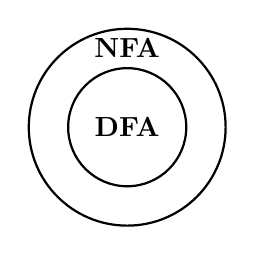
\begin{tikzpicture}
        % Cerchi per gli automi
        \draw[thick] (0, 0) circle (0.75cm) node[pos=0, yshift=0cm] {\textbf{DFA}};
        \draw[thick] (0, 0) circle (1.25cm) node[pos=0, yshift=1cm] {\textbf{NFA}};
    \end{tikzpicture} 
    \end{center}
    
}

Si vuole ora dimostrare che i \red{DFA sono tanto espressivi quanto gli NFA}, sebbene siano un loro sottoinsieme proprio

\mprop{}{
    Per ogni NFA, è prossibile costruire un DFA ad esso equivalente

}
\dimostrazione{
    Occorre seguire contemporaneamente tutti i possibili cammini alternativi dell'NFA di modo che gli stati del DFA che andranno a costruire sono costituiti sa insiemi di stati dell'NFA
}
Per dimostrare questa cosa occorre prima introdurre diversi concetti

\subsubsection{$\epsilon$-closure}

\dfn{$\epsilon$-closure}{
    L'\(\epsilon\)-closure di uno stato \(q \in Q\), denotata come \(\epsilon\text{-closure}(q)\), è definita come l'insieme degli stati \(q'\) tali che esiste un cammino da \(q\) a \(q'\) usando solo transizioni \(\epsilon\), inclusivamente \(q\) stesso.

    In simboli:
    \[
        \epsilon\text{-closure}(q) = \{ q' \in Q \mid q \xrightarrow{\epsilon^*} q' \},
    \]

    In altre parole si puo defnire come il minimo insieme che rispetta le seguenti regole:
    \[
        \frac{}{\{q\}\subseteq \epsilon\text{-closure}(q)}\quad\frac{p\in \epsilon\text{-closure}(q)}{\delta(p,\epsilon)\subseteq \epsilon\text{-closure}(q)}    
    \]

}
nel caso abbiamo un insieme $P$ di nodi allarghiamo la definizione di $\epsilon\text{-closure}$ a quella di:
\[
    \epsilon\text{-closure}(P) = \bigcup_{p\in P}\epsilon\text{-closure}(p)
\]

\esempio{
    Considera il seguente NFA:
    \begin{itemize}
        \item Stati: \(Q = \{q_0, q_1, q_2\}\)
        \item Transizioni:
        \begin{itemize}
            \item \(\delta(q_0, \epsilon) = \{q_1\}\)
            \item \(\delta(q_1, \epsilon) = \{q_2\}\)
            \item \(\delta(q_2, a) = \{q_2\}\)
        \end{itemize}
    \end{itemize}
    Il calcolo dell'\(\epsilon\)-closure è presto fatto:
    \begin{itemize}
        \item \(\epsilon\text{-closure}(q_0)\):
        \begin{itemize}
            \item Da \(q_0\), puoi raggiungere \(q_1\) attraverso una transizione \(\epsilon\)
            \item Da \(q_1\), puoi raggiungere \(q_2\) attraverso un'altra \(\epsilon\)
        \end{itemize}
        Quindi: \(\epsilon\text{-closure}(q_0) = \{q_0, q_1, q_2\}\)
        \item  \(\epsilon\text{-closure}(q_1)\):
        \begin{itemize}
            \item  Da \(q_1\), puoi raggiungere \(q_2\) attraverso una transizione \(\epsilon\)
        \end{itemize}
        Quindi: \(\epsilon\text{-closure}(q_1) = \{q_1, q_2\}\)
        \item \(\epsilon\text{-closure}(q_2)\):
        \begin{itemize}
            \item \(q_2\) non ha transizioni \(\epsilon\) in uscita
        \end{itemize}
        Quindi: \(\epsilon\text{-closure}(q_2) = \{q_2\}\)
    \end{itemize}

}

Qui è presentato l'algoritmo per calcolare la $\epsilon$-closure:
\begin{algorithm}
    \caption{$\epsilon$-closure}
    \KwIn{Stato $p$}
    \KwOut{insieme di stati raggiungibili da $p$ con mosse $\epsilon$}

    $T\gets P$\tcp*{inizalizzazione}
    $\epsilon$-closure($p$) = P\tcp*{inizalizzazione}

    \While{$T\neq \varnothing$}{
        scegli un $r\in T$ e rimuovilo da $T$\;
        \ForEach{$s\in\delta(r,\epsilon)$}{
            \If{$s\neq\epsilon$-closure($p$)}{
                add $s$ to $\epsilon$-closure($p$)\;
                add $s$ to T\;
            }
        }
    }
\end{algorithm} 
\clm{}{}{
    usando le $\epsilon$-closure. si può definire il linguaggio riconosciuto da un NFA in modo elegante. 
    
    Definiamo la seguente funzione
    \[
        \hat{\delta}:Q\times \Sigma^* \mathcal{Q}(P)
    \]
    per in induzione
    \[
        \hat{\delta}(q,\epsilon) = \epsilon\text{-closure}(q)
    \]
    \[
        \hat{\delta}(q,xa) = \epsilon\text{-closure}(q) \text{ dove }P=\{p\in Q\mid \exists r\in \hat{\delta}(q,x)\land p\in (r,a)\}
    \]
    

    Pertanto si può dimostrare (dimostrazione difficile) che:
    \[
        w\in L[N] \iff \exists p \in F t.c. p\in \hat{\delta}(q_0,w)
    \]
}
\subsubsection{funzione mossa}
\dfn{
    funzione mossa
}{
    Si definisce la \textbf{funzione mossa} come estensione della funzione di transizione $\delta$ di un NFA come:
    \[
        \begin{array}{l}
            mossa:\mathcal{P}(Q)\times \Sigma\to \mathcal{P}(Q)\\
            mossa(P,a) = \bigcup_{p\in P}\delta (p,a)
        \end{array}
    \]
    Cioe l’insieme delle mosse $a$ da un insieme di nodi $P$ e l’unione di tutte le mosse $a$ di ogni nodo dell’insieme. `
}

\subsubsection{funzione transazione}
\dfn{funzione transizione}{
    Si definisce \textbf{transizione} e la si denota con $\Delta$ tale funzione:
    \[ 
        \Delta(A,b)=\epsilon\text{-closure}(mossa(A,b)) 
    \]
    Con $A$ un insieme di stati e $b$ una transizione
}

\subsubsection{costruzione per sottoinsiemi del DFA}
Qua di seguito l’algoritmo per la costruzione di sottoinsiemi, che serve per passare da un NFA a un DFA equivalente

\begin{algorithm}
    \caption{costruzionePerSottoinsiemi()}
    \KwIn{NFA $N=(\Sigma, Q,\delta,q_0,F)$}
    \KwOut{DFA $M_N=(\Sigma,T,\Delta, \epsilon\text{-closure}(q_0), \mathcal{F})$}
    $S\gets\epsilon\text{-closure}(q_0)$\tcp*{stato iniziale del DFA}
    $T=\{S\}$\tcp*{$T$ è il l'insieme degli stati del DFA}
    \While{c'è un $P\in T$ non marcato}{
        marca $P$\;
        \ForEach{$a\in\Sigma$}{
            $R\gets \epsilon\text{-closure}(mossa(P,a))$\;
            \If{$R\notin T$}{
                add $R$ to $T$\tcp*{$R$ non ha marca}
                definisci $\Delta(P,a) = R$\;
        }
    }
}
\end{algorithm}

Definiamo quindi il DFA equivalente:
\dfn{DFA quivalente}{
    Si definisce il DFA equivalente tale automa:
    \[
        M_n = (\Sigma, T,\Delta, \epsilon\text{-closure}(q_0), \mathcal{F})    
    \]
    dove $R\in \mathcal{F}\iff \exists q\in R$ con $q\in F$
}

Si può notare come l'algoritmo che definisce la funzione di transizione (vista poch'anzi) rispetta le limitazioni dei DFA: non ci sono mosse epsilon e per ogni caraere dell’alfabeto esiste una ed
una sola mossa in qualunque stato
\esempio{
    Consideriamo l’NFA seguente (relativo all’espressione regolare $((a|b)^*ab)$:
    \begin{center}
        \begin{tikzpicture}[node distance=1cm]
        \node[state, initial] (q0) {$q_0$};
        \node[state] (q1) [right=of q0] {$q_1$};
        \node[state, accepting] (q2) [right=of q1] {$q_2$};

        % Transizioni
        \path[->]
        (q0) edge[loop above] node {$a$} ()
            edge[loop below] node {$b$} ()
            edge[above] node {$b$} (q1)
        (q1) edge node[above] {$a$} (q2);
    \end{tikzpicture}
    \end{center}
    

    Vogliamo ora trovare un DFA equivalente ad esso, applichiamo l’algoritmo di costruzioni per sottoinsiemi:
    \begin{itemize}
        \item calcoliamo lo stato iniziale $S=\epsilon\text{-closure}(q_0)$, che è $S=q_0$. 
        \item Creiamo $T$ e gli inseriamo $S$ marcandolo
        \item Per ogni simbolo dobbiamo calcolare $\epsilon\text{-closure}(mossa(P,a))$, ma visto che l'alfabeto è $\{a,b\}$ lo facciamo 2 volte:
        \begin{itemize}
            \item per il carattere $a$ calcoliamo con $P=S=\{q_0\}$:
              \[
                \begin{array}{l}
                    R = \epsilon\text{-closure}(mossa(P,a)) = \epsilon\text{-closure}\left(\bigcup_{p\in\{q_0\}}\delta (p,a)\right)\\
                    =\epsilon\text{-closure}(\delta(q_0,a)) =\epsilon\text{-closure}(\{q_0\}) =\{q_0\}
                \end{array}
              \]
                 
            Si definisca $\delta(S,a)=\{q_0\}$ e visto che $\{q_0\}\in T$ non lo andiamo a ri-aggiungere
            \item per il carattere $a$ calcoliamo con $P=S=\{q_0\}$:
              \[
                \begin{array}{l}
                    R = \epsilon\text{-closure}(mossa(P,b)) = \epsilon\text{-closure}\left(\bigcup_{p\in\{q_0\}}\delta (p,b)\right) \\                
                    =\epsilon\text{-closure}(\delta(q_0,b)) =\epsilon\text{-closure}(\{q_0, q_1\}) =\{q_0,q_1\}
                \end{array}
              \]
            visto che $\{q_0,q_1\}\notin T$ lo andiamo ad aggiungere
        \end{itemize}
        \item si calcoli ora con $P=\{q_0, q_1\}$ andando a calcolare la stessa cosa:
        \begin{itemize}
            \item per $a$ si ha:
              \[
                \begin{array}{l}
                    R=    \epsilon\text{-closure} (mossa(P,a)) = \epsilon\text{-closure}\left(\bigcup_{p\in\{q_0, q_1\}}\delta(p,a)\right)\\                 
                    = \epsilon\text{-closure} (\{q_0\}\cup\{ q_2\}) = \{q_0,q_2\}
                \end{array}
              \]
            quindi $\Delta(\{q_0,q_1\}, a)=\{q_0,q_2\}$. Visto $\{q_0,q_2\}\notin T$ lo aggiungiamo 
            \item  per $b$ si ha $R=\{q_0,q_1\}$. Quindi $\Delta(\{q_0, q_1\}, b) = \{q_0,q_1\}$ e non lo si raggiunge
        \end{itemize}
        \item ripetiamo per $P=\{q_0, q_2\}$ (salto i calcoli)
    \end{itemize}

    alla fine di sto ambaradam si ottiene $DFA \;N'=(\Sigma, \{\{q_0\},\{q_0,q_1\}, \{q_0,q_2\}\}, \Delta, \{q_0\}, \{q_0,q_2\})$ che in forma di diagramma di transizione e:
    \begin{center}
        \begin{tikzpicture}[shorten >=1pt, node distance=3cm, on grid, auto]

            % Stati
            \node[state, initial] (q0) {$A=\{q_0\}$};
            \node[state] (q1) [right=of q0] {$B=\{q_0, q_1\}$};
            \node[state, accepting] (q2) [below=of q1] {$C=\{q_0, q_2\}$};
        
            % Transizioni
            \path[->]
                (q0) edge[loop above] node {$a$} () % loop su q0 con "a"
                     edge[bend left] node {$b$} (q1) % da q0 a q1 con "b"
                (q1) edge[loop above] node {$b$} () % loop su q1 con "b"
                     edge[bend left] node {$a$} (q2) % da q1 a q2 con "a"
                (q2) edge[bend left] node {$b$} (q1) % da q2 a q1 con "b"
                     edge[bend left] node {$a$} (q0); % da q2 a q0 con "a"
        
        \end{tikzpicture}
            \end{center}
}

esempio bello corposo:
\esempio{
    \begin{center}
        \begin{tikzpicture}[shorten >=1pt, node distance=2cm, on grid, auto]
            % Stati
            \node[state, initial] (q0) {$q_0$};
            \node[state] (q2) [right of=q0] {$q_2$};
            \node[state, accepting] (q4) [right of=q2] {$q_4$};
            \node[state] (q1) [above of=q1] {$q_1$};
            \node[state] (q3) [right of=q1] {$q_3$};
        
            % Transizioni
            \path[->]
                (q0) edge[bend left] node {$\epsilon$} (q1)
                     edge node[below] {$b$} (q2)
                (q1) edge node {$a$} (q0)
                     edge node {$\epsilon$} (q2)
                     edge node {$\epsilon$} (q3)
                     edge node {$a$} (q4)
                (q2) edge node[below] {$b$} (q4)
                (q3) edge[bend left] node {$a$} (q4)
                (q4) edge[bend left] node {$\epsilon$} (q3);
        \end{tikzpicture}
        \end{center}
        
        si noti i seguenti calcoli

        \vspace{0.5cm}
        \begin{math}
            A = \epsilon\text{-closure}(q_0) = \{q_0, q_1, q_2, q_3\} \\
            \Delta(A, a) = \epsilon\text{-closure}(\text{move}(A, a)) = \epsilon\text{-closure}(\{q_0, q_4\}) = \{q_0, q_1, q_2, q_3, q_4\} = B \\
            \Delta(A, b) = \epsilon\text{-closure}(\text{move}(A, b)) = \epsilon\text{-closure}(\{q_2, q_3, q_4\}) = \{q_2, q_3, q_4\} = C \\
            \Delta(B, a) = \epsilon\text{-closure}(\text{move}(B, a)) = \epsilon\text{-closure}(\{q_0, q_4\}) = B \\
            \Delta(B, b) = \epsilon\text{-closure}(\text{move}(B, b)) = \epsilon\text{-closure}(\{q_2, q_4\}) = C \\
            \Delta(C, a) = \epsilon\text{-closure}(\text{move}(C, a)) = \epsilon\text{-closure}(\{q_4\}) = \{q_3, q_4\} = D \\
            \Delta(C, b) = \epsilon\text{-closure}(\text{move}(C, b)) = \epsilon\text{-closure}(\{q_4\}) = D \\
            \Delta(D, a) = \epsilon\text{-closure}(\text{move}(D, a)) = \epsilon\text{-closure}(\{q_4\}) = \varnothing = D \\
            \Delta(D, b) = \epsilon\text{-closure}(\text{move}(D, b)) = \epsilon\text{-closure}(\varnothing) = \varnothing = E \\
            \Delta(E, a) = \epsilon\text{-closure}(\text{move}(E, a)) = \epsilon\text{-closure}(\varnothing) = \varnothing = E \\
            \Delta(E, b) = \epsilon\text{-closure}(\text{move}(E, b)) = \epsilon\text{-closure}(\varnothing) = \varnothing = E
        \end{math}
        \vspace{0.5cm}

        il cui DFA $M_N$ è:
        
        \begin{center}
        \begin{tikzpicture}[shorten >=1pt, node distance=2cm, on grid, auto]
            % Stati
            \node[state, initial] (A) {$A$};
            \node[state, accepting] (B) [above right=of A] {$B$};
            \node[state, accepting] (C) [below right=of A] {$C$};
            \node[state, accepting] (D) [right=of C] {$D$};
            \node[state] (E) [right=of D] {$E$};
        
            % Transizioni
            \path[->]
                (A) edge[above] node {$a$} (B)
                    edge[above] node[below] {$b$} (C)
                (B) edge[loop above] node {$a$} ()
                    edge node[left] {$b$} (C)
                (C) edge[below] node {$a,b$} (D)
                (D) edge[above] node {$b$} (E)
                    edge[loop above] node {$a$} ()
                (E) edge[loop above] node {$a, b$} ();
        \end{tikzpicture}
        \end{center}
}

\subsubsection{casi pessimi}

\clm{}{
    Vi sono tuttavia casi pessimi in cui il DFA equivalente è esponenzialmente più grande di del DFA, ovvero che se il NFA $N$ ha $n$ stati il suo $M_n$ può averne $2^n$
}

\esempio{
        Sia $N$ il seguente NFA con 2 stati:
        \begin{center}
            \begin{tikzpicture}
            \node[state, initial] (q0) {$q_0$};
            \node[state, accepting] (q1) [right=of q0] {$q_1$};

            \path[->]
                (q0) 
                    edge node[below] {$b$} (q1)
                    edge[loop below] node {$b$} ()
                    edge[loop above] node {$a$} ()
                (q1) 
                    edge[loop above] node {$c$} (); 
        \end{tikzpicture}
        \end{center}
        

        per costruire il suo $M_N$ si hanno i seguenti nodi
        \begin{itemize}
            \item $A=\{q_0\}$
            \item $B=\{q_0, q_1\}$
            \item $A=\{q_1\}$
            \item $D=\varnothing$
        \end{itemize} 

        in diagramma di transazione diventa:
        \begin{center}
            \begin{tikzpicture}[node distance=1cm]
            \node[state, initial] (a) {$A$};
            \node[state, accepting] (b) [right=of a] {$B$};
            \node[state] (d) [below=of a] {$D$};
            \node[state, accepting] (c) [right=of d] {$C$};

            \path[->]
                (a) 
                    edge[bend left] node[below] {$b$} (b)
                    edge[loop above] node {$a$} ()
                    edge[above] node[left] {$c$} (d)
                (b) 
                    edge[loop above] node {$b$} ()
                    edge[above] node[left] {$c$} (c)
                    edge[bend left] node[below] {$a$} (a)
                (d) 
                    edge[loop below] node {$a,b,c$} ()
                (c) 
                    edge[loop below] node {$c$} ()
                    edge[bend right] node[above] {$b$} (d)
                    edge[bend left] node[below] {$a$} (d);
        \end{tikzpicture}
        \end{center}
        

}



Adesso si può dimostrare il teorema dell'equivalenza
\subsubsection{teorema d'equivalenza tra NFA e DFA}

\thm{
    Bonzo-GioLaPalma
}{
    Sia $N=(\Sigma, Q,\delta,q_0, F)$ un NFA  e sia $M_n$ l'automa ottenuto con la costruzione per sottoinsiemi. allora $M_n$ è un DFA e si ha che 
    \[
        L[N]=L[M_n]    
    \]
    In altre parole, $ N $ e $ M_n $ sono equivalenti.
}
\dimostrazione{
    Sia \( N = (Z, \Sigma, \delta, q_0, F) \) un NFA e sia \( M_N = (\Gamma, \Sigma, \Delta, A, F') \) l'automa ottenuto con l'algoritmo.

\begin{itemize}
    \item \( M_N \) è \textbf{deterministico}: Infatti $\Delta(A, a)$ con $A\in T\land a\in \Sigma$ è definita in modo univoco 
        

    \item  Quindi mi riduco a dimostrare che $L[N]=L[M_n]$
    \begin{itemize}
        \item si osservi che per un DFA, $\epsilon$-closure$(R)=R$
        \item chiamiamo $i_m=\epsilon$-closure$(q_0)$ lo stato iniziale di $M_n$
    \end{itemize}
\end{itemize}



Vogliamo dimostrare che $\forall w\in \Sigma^*$

\[
\delta(q_0, w) = \Delta(A, w) 
\]
per induzione sulla lunghezza di $w$
\begin{itemize}
    \item \textbf{Caso base}: \( |w| = 0 \text{ cioè } w=\epsilon \):
    \[
        \hat{\delta}(A, \epsilon) = \epsilon\text{-closure}(q_0)
    \]
    \[
        \hat{\Delta} (i_m,\epsilon) =     \epsilon\text{-closure}(i_m)= i_M=<\epsilon\text{-closure}(q_0)
    \]
    \item \textbf{Caso induttivo}:\( w = xa \) con \( x \in \Sigma^*, a \in \Sigma \)
    Per ipotesi induttiva, sappiamo che:
    \[
        \hat{\delta}(q_0, x) = \Delta(\{q_0\}, x) = \{p_1, \dots, p_k\}
    \]
    
    Per definizione di \(\hat{\delta}\):
    \[
        \hat{\delta}(q_0, xa) = \Delta\big(\varepsilon\text{-closure}\big(\bigcup_{i=1}^{k} \delta(p_i, a)\big)\big)
    \]
    
    Similmente:
    \[
        \Delta(\{q_0\}, xa) = \Delta(\{p_1, \dots, p_k\}, a)
    \]
    
    In base all'algoritmo, la definizione di \(\Delta\) ci dice che:
    \[
        \Delta(\{p_1, \dots, p_k\}, a) = \varepsilon\text{-closure}\big(\text{mossa}(\{p_1, \dots, p_k\}, a)\big)= \varepsilon\text{-closure}\big(\bigcup_{i=1}^{k} \delta(p_i, a)\big)= \hat{\delta}(q_0, xa)
    \]
    OK.
    
    ---
    
    Infine, abbiamo che:
    \[
        w \in L[N] \iff \exists p \in \hat{\delta}(q_0, w) \text{ con } p \in F
    \]
    
    \[
        \iff \exists p \in \Delta(i_H, w) \text{ con } p \in F
    \]
    
    \[
        \iff w \in L[M_N] \quad \forall w \in \Sigma^*
    \]
    
    Quindi:
    \[
        L[N] = L[M_N] \quad \text{c.v.d.}
    \]
    
\end{itemize}

}

\subsection{Da espressioni regolarei a NFA equivalenti}

\thm{Basta - Dario è sVenuto}{
    Data un'espressione regolare $S$, possiamo costruire un NFA $N[s]$ tale che:
    \[
        \mathcal{L}[s] = L[N[s]]
    \]

    ovvero un linguaggio individuato da un linguaggio regolare è equivalente ad un linguaggio riconosciuto da un automa non deterministico a stati finiti costruito a partire da $S$, questo significa che \red{gli NFA riconoscono TUTTI i linguaggi regolari}, vedremo poi che riconoscono solo i linguaggi regolari
}
\dimostrazione{
    Dimostreremo il teorema per induzione sulla sintassi astratta della espressione regolare $S$.

    Si costruisca un possibile NFA associato all'espressione regolare $S$, in modo da mantenere i seguente due invarianti:
    \begin{itemize}
        \item lo stato iniziale non ha archi entranti
        \item $N[s]$ ha un solo stato finale senza archi uscenti
    \end{itemize}

    Procedo ad esaminare i vari casi 
    \begin{itemize}
        \item Sia $s=\varnothing$
        
        In questo caso sarà possibile costruire un NFA con due stati (iniziale e finale) non connessi, quindi $N[s]$:
        \begin{center}
            \begin{tikzpicture}
                \node[state, initial] (A) {};
                \node[state, accepting] (B) [right of=A] {};
            \end{tikzpicture}
        \end{center}
        Si osservi che $\mathcal{L}[\varnothing]=\varnothing=L[N[s]]$
        \item Sia $s=\epsilon$
        
        In questo caso sarà possibile costruire un NFA con due stati (iniziale e finale) connessi da un $\epsilon$, quindi $N[s]$:

        \begin{center}
            \begin{tikzpicture}
                \node[state, initial] (A) {};
                \node[state, accepting] (B) [right of=A] {};

                \path[->]
                    (A) edge[above] node{$\epsilon$} (B);
            \end{tikzpicture}


        \end{center}
        Si osservi che, in questo caso, $\mathcal{L}[\epsilon] = \{\epsilon\}=L[N[s]]$
        \item Sia $S = a$
        
        In questo caso sarà possibile costruire un NFA con due stati (iniziale e finale) connessi da una transizione $a$, quindi $N[s]$:

        \begin{center}
            \begin{tikzpicture}
                \node[state, initial] (A) {};
                \node[state, accepting] (B) [right of=A] {};

                \path[->]
                    (A) edge[above] node{$a$} (B);
            \end{tikzpicture}
        \end{center}

        Si osservi che, in questo caso, $\mathcal{L}[a] = \{a\}=L[N[s]]$
        \item caso $s= r|t$
        
        Ipotizziamo di avere già costruito gli automi $N[t]$ ed $N[r]$, per costruire "l'or" è possibile partire da uno stato iniziale $i$ e collegarlo con transizioni $\epsilon$ ai due automi, da entrambi si confluisce in uno stato finale $f$ con transazioni $\epsilon$
        
        \begin{center}
            \begin{tikzpicture}[shorten >=1pt, node distance=2cm, on grid, auto]
                % Stati
                \node[state, initial] (qi) {$q_i$};
                \node[state] (ir) [above right=of qi] {$i_r$};
                \node[state] (fr) [right=of ir] {$f_r$};
                \node[state] (it) [below right=of qi] {$i_t$};
                \node[state] (ft) [right=of it] {$f_t$};
                \node[state, accepting] (qf) [right=5cm of qi] {$q_f$};
            
                % Transizioni
                \path[->]
                (qi) edge[above] node {$\varepsilon$} (ir)
                     edge[below] node {$\varepsilon$} (it)
                (ir) edge[above] (fr)
                (fr) edge[above] node {$\varepsilon$} (qf)
                (it) edge[above] (ft)
                (ft) edge[below] node {$\varepsilon$} (qf);

                %TODO inserire cerchi per contenere gli automi
                
            \end{tikzpicture}
            
        \end{center}

        Algebricamente si può dimostrare che $\mathcal{L}[r|t]=\mathcal{L}[t]\cup \mathcal{L}[r]$

        e per ipotesi induttiva si ha:
        \[
            \mathcal{L}[t]\cup \mathcal{L}[r] =L[N[r]]\cup L[N[t]] =L[N[r|t]]
        \]
        \item Sia $s=r\cdot t$
        
        Ipotizziamo di avere già costruito gli automi $N[t]$ ed $N[r]$, per costruire la concatenazione è possibile fondere lo stato finale del primo automa con quello del secondo automa, si ha, quindi, che $N[s]$:

        \begin{center}
            \begin{tikzpicture}
                [shorten >=1pt, node distance=2cm, on grid, auto]
                % Stati
                \node[state, initial] (ir) {$q_i$};
                \node[state] (frit) [right=of ir] {$f_r = i_t$};
                \node[state, accepting] (ft) [right=of frit] {$f_t$};
                
                % Transizioni
                \path[->]
                    (ir) edge (frit)
                    (frit) edge (ft);
            \end{tikzpicture}            
        \end{center}

        %TODO inserire cerchi per gli automi probabile libreria FIT

        \item Sia $s=r^*$
        
        Ipotizzando di aver già costruito $N[r]$ è possibile costruire l'automa creando un ciclo $\epsilon$ dalla fine di $N[r]$ al suo inizio

        \begin{center}
            \begin{tikzpicture}
                [shorten >=1pt, node distance=2cm, on grid, auto]
                % Stati
                \node[state, initial] (i) {$i$};
                \node[state] (it) [right=of i] {$i_r$};
                \node[state] (ft) [right=of it] {$f_r$};
                \node[state, accepting] (f) [right=of ft] {$f$};

                
                % Transizioni
                \path[->]
                    (i) edge node {$\epsilon$} (it)
                        edge[bend left] node {$\epsilon$} (f)
                    (it) edge (ft)
                    (ft) 
                        edge node {$\epsilon$} (f)
                        edge[bend left] node {$\epsilon$} (it);
                    
            \end{tikzpicture}            
        \end{center}

        Si osservi che:

        \[
            \mathcal{L}[r^*] = (\mathcal{L}[r])^* 
        \]
        per ipotesi induttiva

        \[
            (\mathcal{L}[r])^* = (L[N[r]])^* = L[N[r^*]]
        \]
    \end{itemize}
}
\esempio{
    Sia $S= (a|b^*)ba$ un'espressione regoalre e costruiamnone l'albero sintattico

    \begin{center}
       \begin{tikzpicture}
        \Tree[
                .$\cdot$
                [
                    .$*$
                    [
                        .$|$
                        a
                        b
                    ]
                ]
                [
                    .$\cdot$
                    b
                    a
                ]
        ]
    \end{tikzpicture} 
    \end{center}

    Partiamo dalle foglie e risaliamo alla radice (bottom-up)
    Si ha:

    \begin{itemize}
        \item $N[a]$:
        \begin{center}
            \begin{tikzpicture}
                \node[state, initial] (A) {};
                \node[state, accepting] (B) [right of=A] {};

                \path[->]
                    (A) edge[above] node{$a$} (B);
            \end{tikzpicture}
        \end{center}

        \item $N[b]$:
        \begin{center}
            \begin{tikzpicture}
                \node[state, initial] (A) {};
                \node[state, accepting] (B) [right of=A] {};

                \path[->]
                    (A) edge[above] node{$b$} (B);
            \end{tikzpicture}
        \end{center}

        \item  $N[a|b]$:
        
        \begin{center}
            \begin{tikzpicture}[shorten >=1pt, node distance=2cm, on grid, auto]
                % Stati
                \node[state, initial] (qi) {};
                \node[state] (ir) [above right=of qi] {};
                \node[state] (fr) [right=of ir] {};
                \node[state] (it) [below right=of qi] {};
                \node[state] (ft) [right=of it] {};
                \node[state, accepting] (qf) [right=5cm of qi] {};
            
                % Transizioni
                \path[->]
                (qi) edge[above] node {$\varepsilon$} (ir)
                     edge[below] node {$\varepsilon$} (it)
                (ir) edge[above] node {$a$} (fr)
                (fr) edge[above] node {$\varepsilon$} (qf)
                (it) edge[above] node {$b$} (ft)
                (ft) edge[below] node {$\varepsilon$} (qf);

                %TODO inserire cerchi per contenere gli automi
                
            \end{tikzpicture}
            
        \end{center}

        \item  $N[(a|b)^*]$:
        
        \begin{center}
            \begin{tikzpicture}[shorten >=1pt, node distance=2cm, on grid, auto]
                % Stati
                \node[state, initial] (i) {};
                \node[state] (qi) [right=of i] {};
                \node[state] (ir) [above right=of qi] {};
                \node[state] (fr) [right=of ir] {};
                \node[state] (it) [below right=of qi] {};
                \node[state] (ft) [right=of it] {};
                \node[state] (qf) [right=5cm of qi] {};
                \node[state, accepting] (f) [right=of qf] {};
            
                % Transizioni
                \path[->]
                (i) edge[above] node {$\epsilon$} (qi)
                (qi) edge[above] node {$\varepsilon$} (ir)
                     edge[below] node {$\varepsilon$} (it)
                (ir) edge[above] node {$a$} (fr)
                (fr) edge[above] node {$\varepsilon$} (qf)
                (it) edge[above] node {$b$} (ft)
                (ft) 
                    edge[below] node {$\varepsilon$} (qf)
                    
                (qf) edge[below] node {$\epsilon$} (f)
                    edge[below] node {$\varepsilon$} (qi);

            \end{tikzpicture}
            
        \end{center}
        \item $N[ba]$:
        \begin{center}
            \begin{tikzpicture}
                \node[state, initial] (A) {};
                \node[state] (B) [right=of A] {};
                \node[state, accepting] (C) [right=of B] {};

                \path[->]
                    (A) edge[above] node{$b$} (B)
                    (B) edge[above] node{$a$} (C);
            \end{tikzpicture}
        \end{center}

        \item $N[s]$:
        \begin{center}
            \begin{tikzpicture}[shorten >=1pt, node distance=2cm, on grid, auto]
                % Stati
                \node[state, initial] (i) {};
                \node[state] (qi) [right=of i] {};
                \node[state] (ir) [above right=of qi] {};
                \node[state] (fr) [right=of ir] {};
                \node[state] (it) [below right=of qi] {};
                \node[state] (ft) [right=of it] {};
                \node[state] (qf) [right=5cm of qi] {};
                \node[state] (f) [right=of qf] {};
                \node[state] (B) [right=of f] {};
                \node[state, accepting] (C) [right=of B] {};
            
                % Transizioni
                \path[->]
                (i) edge[above] node {$\epsilon$} (qi)
                (qi) edge[above] node {$\varepsilon$} (ir)
                     edge[below] node {$\varepsilon$} (it)
                (ir) edge[above] node {$a$} (fr)
                (fr) edge[above] node {$\varepsilon$} (qf)
                (it) edge[above] node {$b$} (ft)
                (ft) 
                    edge[below] node {$\varepsilon$} (qf)
                    
                (qf) 
                    edge[below] node {$\epsilon$} (f)
                    edge[below] node {$\varepsilon$} (qi)
                (f) edge[above] node{$b$} (B)
                (B) edge[above] node{$a$} (C);

            \end{tikzpicture}
            
        \end{center}


        
    \end{itemize}

    


}

Altro esempietto:
\esempio{
        TODO da fare l'automa diretto qui

\[
\begin{aligned}
    &\text{Costruiamo il DFA associato a } N[s]: \\
    &A = \varepsilon\text{-closure}(0) = \{0\} \\
    &\Delta(A, a) = \varepsilon\text{-closure}(\{1\}) = \{1, 2, 3\} = B \\
    &\Delta(A, b) = \varepsilon\text{-closure}(\varnothing) = \varnothing = C \\
    &\Delta(B, a) = \varepsilon\text{-closure}(\{5\}) = \{5\} = D \\
    &\Delta(B, b) = \varepsilon\text{-closure}(\{3\}) = \{3, 4, 2\} = E \\
    &\Delta(D, a) = \varnothing = C, \quad \Delta(D, b) = \varnothing = C \\
    &\Delta(E, a) = \varepsilon\text{-closure}(\{5\}) = D, \quad \Delta(E, b) = \varepsilon\text{-closure}(\{3\}) = E \\
    &\Delta(C, a) = \varnothing = C, \quad \Delta(C, b) = \varnothing = C
\end{aligned}
\]

\begin{tikzpicture}[shorten >=1pt, node distance=0.5cm, on grid, auto]
    % Stati
    \node[state, initial] (A) {$A$};
    \node[state] (B) [above right=of A] {$B$};
    \node[state, accepting] (D) [below right=of A] {$D$};
    \node[state] (C) [below of=D] {$C$};
    \node[state] (E) [right=of B] {$E$};

    % Transizioni
    \path[->]
        (A) edge node {$a$} (B)
            edge[bend right] node[below] {$b$} (C)
        (B) edge node {$a$} (D)
            edge[bend left] node[above] {$b$} (E)
        (D) edge[loop below] node {$a,b$} (D)
        (C) edge[loop below] node {$a,b$} (C)
        (E) edge[loop above] node {$b$} (E)
            edge[bend left] node {$a$} (D);
\end{tikzpicture}

\[
\text{DFA associato a } N[a \; b^* \; a]
\]

}

\subsection{Da NFA a espressione regolare}
Aggiungo una dimostrazione presa dal libro di Michael Sipser, "Introduction to the Theory of Computation", che descrive come creare un'espressione regolare partendo direttamente da un NFA. Nella sezione successiva introdurremo le grammatiche regolari con le quali e' possibile dimostrare lo stesso teorema, quindi questa parte non e' necessaria ma solo un'idea interessante e piu' diretta.

Come anticipato precedentemente, e' possibile anche dimostrare la direzione inversa del teorema, ovvero che dato un NFA che riconosce un linguaggio $ L[N] $, e' sempre possibile generare un'espressione regolare che riconosca lo stesso linguaggio. Quindi vale il teorema generale:
\thm{Teoremone Piccolomini}{
  Un linguaggio e regolare sse esiste un automa a stati finiti che lo riconosce.
}
Sopra abbiamo gia dimostrato che preso un linguaggio regolare (ovvero descritto da un'espressione regolare) possiamo sempre costruire un NFA equivalente. Ci tocca dimostrare la direzione inversa, ovvero che preso un qualsiasi NFA, il linguaggio che riconosce e' regolare e quindi esiste un'espressione regolare che lo descrive.

Dato che abbiamo dimostrato col teorema Bonzo-GiolaPalma che un NFA e' sempre convertibile a un DFA, possiamo partire proprio da un DFA e definire un procedimento per ottenere un'espressione regolare equivalente. Dividiamo in due parti questo processo: prima convertiamo il DFA in un GNFA (General Nondeterministic Finite Automata), che ora defineremo, poi convertiamo il GNFA in un'ER.

\subsubsection{Automi finiti nondeterministici generali}
I GNFA sono praticamente dei NFA con funzione di transizione che funziona utilizzando le ER. Possono leggere blocchi alla volta dall'input, non solo caratteri, e se tale blocco soddisfa l' ER di una transizione che parte dallo stato corrente, allora si puo' seguire l'arco e cambiare stato. Ovviamente e' fortemente nondeterministico e possono esserci molti modi per elaborare la stessa sequenza di caratteri. 

TODO: esempio di GNFA

Formalmente:
\dfn{GNFA}{
  Un \textbf{automa finito nondeterministico generale} e' una quintupla $ (Q, \Sigma, \delta, q_{\text{start}}, q_{\text{accept}}) $ tale che:
  \begin{itemize}
    \item $ Q $ e' un insieme finito di stati
    \item $ \Sigma $ e' l'alfabeto dell'input
    \item $ \delta: (Q - q_{\text{accept}}) \times (Q - q_{\text{start}}) \to \mathcal{R}_\Sigma $ e' la funzione di transizione
  \end{itemize}
  
  Dove $ \mathcal{R}_\Sigma $ e' l'insieme di tutte le ER sull'alfabeto $ \Sigma $.
}
 
Un GNFA riconosce una stringa $ w \in \Sigma^* $ se esitono una suddivisione $ w = w_1w_2...w_k $ con $ w_i \in \Sigma^* $ e una serie di stati $ q_0,q_1,...,q_k $ tali che:
\begin{enumerate}
  \item $ q_0 = q_{\text{start}} $
  \item $ q_k = q_{\text{accept}} $
  \item $ \forall i > 0. w_i \in \mathcal[R_i] $, dove $ R_i = \delta(q_{i-1}, q_i) $
\end{enumerate}


Per i fini della dimostrazione, ci interessiamo solo di GNFA specifici che rispettano le seguenti condizioni:
\begin{itemize}
  \item Lo stato iniziale ha archi che vanno verso tutti gli altri stati, ma nessuno entrante.
  \item Lo stato finale e' unico e ha archi entranti da tutti gli altri stati, ma nessuno uscente. Inoltre e' distinto dallo stato iniziale.
  \item Senza contare lo stato iniziale e lo stato finale, gli stati hanno archi che vanno verso tutti gli altri stati e anche verso loro stessi.
\end{itemize}

\subsubsection{Da DFA a GNFA}
Convertire un DFA in un GNFA in forma speciale e' semplice: basta aggiungere uno stato iniziale con arco $ \epsilon $ verso lo stato iniziale vecchio, aggiungere uno stato finale con archi $ \epsilon $ entranti da tutti i vecchi stati finali e se ce piu' di un arco nella stessa direzione fra due nodi, fonderli insieme creando un unico arco la cui ER corrispondente e' l'unione delle ER dei vecchi archi. Infine, se mancano degli archi, aggiungere transizioni segnati dall'ER $ \emptyset $, che non puo' essere mai usata. 

\subsubsection{Da GNFA a ER}
Per ottenere l'ER a partire dal GNFA, l'idea principale e' la seguente:\\
Diciamo che il GNFA ha $ k $ stati. Sappiamo che $ k \geq 2 $ perche ci devono essere uno stato finale e uno iniziale distinti. Se riusciamo a rimuovere uno stato alla volta, che non sia finale o iniziale, mantenendo il nuovo GNFA appena ottenuto equivalente a quello prima, arriviamo ad un punto dove $ k=2 $ e l'automa e' costituito semplicemente da un arco che applica l'ER che ci porta dallo stato iniziale direttamente a quello finale, e che descrive quindi il linguaggio riconosciuto dal DFA iniziale.

Dobbiamo fare in modo che quando uno stato $ q_{\text{rip}} $ viene rimosso, le ER sugli archi vengano modificate in modo da simulare tutti i percorsi che sono stati rimossi. Quindi le nuove ER devono considerare sia le stringhe che portano direttamente dallo stato $ q_i $ allo stato $ q_j $, che le stringhe che portavano da $ q_i $ a $ q_j $ passando da $ q_{\text{rip}} $.

TODO: copia figure 1.63 del libro

Quindi, se nel vecchio GNFA:
\begin{enumerate}
  \item $ q_i $ va da $ q_{\text{rip}} $ per l'ER $ R_1 $
  \item $ q_{\text{rip}} $ va a se stesso per $ R_2 $
  \item $ q_{\text{rip}} $ va a $ q_j $ per $ R_3 $
  \item $ q_i $ va a $ q_j $ per $ R_4 $
\end{enumerate}
allora nel nuovo GNFA dobbiamo etichettare l'arco da $ q_i $ a $ q_j $ con l'ER:
\[
  (R_1)(R_2)^*(R_3)\cup (R_4)
\]
Ad ogni iterazione applichiamo questa trasformazione per ogni arco fra una coppia $ q_i q_j $ (anche quando $ i = j $). Formalizziamo tutto cio' (zio perone):
\pf{Dimostrazione formale}{
  Sia $ M $ il DFA equivalente all'NFA del teorema. Usando la procedura descritta sopra trasformiamo $ M $ in un GNFA $ G $. Usiamo la procedura ricorsiva CONVERT($ G $) per ottenere l'ER equivalente:
  \begin{enumerate}
    \item Sia $ k $ il numero di stati di $ G $
    \item Se $ k = 2 $, ritorna l'espressione regolare associata ai due nodi
    \item Se $ k > 2 $, seleziona uno stato $ q_{\text{rip}} \in Q $ che sia diverso dallo stato iniziale e finale e sia $ G' = (Q', \Sigma, \delta', q_{\text{start}}, q_{\text{accept}}) $ tale che:
      \begin{itemize}
        \item $ Q' = Q \setminus \{q_{\text{rip}}\} $
        \item $ \forall q_i \in Q' \setminus \{q_{\text{start}}\}, \forall q_j \in Q' \setminus \{q_{\text{accept}}\}: $
          \[
            \delta'(q_i, q_j) = (R_1)(R_2)^*(R_3)\cup(R_4)
          \]
          con $ R_1 = \delta(q_i, q_{\text{rip}}), R_2 = \delta(q_{\text{rip}}, q_{\text{rip}}), R_3 = \delta(q_{\text{rip}}, q_j), R_4 = \delta(q_i, q_j) $
      \end{itemize}
  \end{enumerate}

  Ora dimostriamo che CONVERT($ G $) ritorni il valore corretto. 

  Dimostriamo per induzione su $ k $, il numero di stati del GNFA $ G $:
  \begin{itemize}
    \item \textbf{Caso base:}

      Se $ k = 2 $, per la definizione di GNFA specifico abbiamo uno stato iniziale e un arco che lo collega allo stato finale. L'ER dell'arco descrive tutte le stringhe che portano $ G $ allo stato finale, quindi e' equivalente a $ G $.
    \item \textbf{Caso induttivo su $ k $:}

      Assumiamo che CONVERT($ G' $) equivale a $ G' $, dove $ G' $ e' il caso con $ k-1 $ stati. Dimostriamo che $ G' $ e $ G $ sono equivalenti. Prendiamo una parola $ w \in \Sigma^* $ accettata da $ G $. Quindi siano
      \[
      q_{\text{start}}, q_1, q_2, q_3, ..., q_{\text{accept}}
      \]
      la sequenza di stati di $ G $ di un percorso che accetta $ w $. Se $ q_{\text{rip}} $ (lo stato rimosso da $ G $ per creare $ G' $) non appartiene a questa sequenza, allora chiaramente $ w $ e' riconosciuto anche da $ G' $. Questo e' perche' i nuovi archi fra tutti gli stati mantengono l'ER originale tramite un'unione. Altrimenti, se $ q_{\text{rip}} $ fa parte del percorso, basta rimuovere tutte le evenienze dalla sequenza per trovare un percorso per cui $ G' $ accetta $ w $. Questo e' perche' nella definizione di CONVERT, facciamo in modo che le nuove ER fra due nodi considerino descrivino anche tutte le stringhe che portavano fra i due stati passando da $ q_{\text{rip}} $. 

      Al contrario, se $ G' $ riconosce $ w $, ad ogni arco e' associata un'ER che riconosce stringhe che in $ G $ fanno passare da $ q_i $ a $ q_i $ sia direttamente che tramite $ q_{\text{rip}} $. Quindi ovviamente anche $ G $ riconosce $ w $. Avendo dimostrato che $ G $ e $ G' $ sono equivalenti, possiamo usare l'ipotesi induttiva per dire che CONVERT($ G $) equivale a $ G $.
  \end{itemize}
}


\subsection{Chiusura dei linguaggi regolari rispetto alle operazioni regolari}
Per aiutarci ad architettare automi finiti o per distinguere linguaggi regolari da altri tipi di linguaggi che vedremo piu' avanti, puo' tornare utile sapere se sono chiusi rispetto alle operazioni regolari (concatenazione, unione, stella di Kleene). Generalmente, diciamo che un'insieme di oggetti e' chiusa rispetto a un'operazione se applicando quest'ultima a qualunque elemento dell'insieme, il risultato appartiene sempre allo stesso insieme. Quindi se consideriamo come macro-insieme l'insieme di tutti i linguaggi regolari e dimostriamo la chiusura rispetto a una certa operazione, allora siamo sicuri che il risultato di questa operazione applicata a linguaggi regolari sara' sempre un linguaggio regolare. Partiamo con l'operazione di unione:
\thm{Chiusura di linguaggi regolari rispetto all'unione}{
  La classe dei linguaggi regolari e' chiusa sotto l'unione.

  In altre parole, se $ A_1 $ e $ A_2 $ sono linguaggi regolari, lo e' anche $ A_1 \cup A_2 $.
}
Dato che abbiamo gia' dimostrato l'equivalenza fra DFA e NFA, possiamo usare il nondeterminismo per dimostrare il teorema sopra (e' possibile anche usare solo DFA, ma e' piu' lunga). L'idea della dimostrazione e' quella di creare due NFA, $ N_1, N_2 $ che riconoscono rispettivamente i linguaggi $ A_1, A_2 $, e poi di unirli per creare un nuovo NFA $ N $ che riconosca $ A_1 \cup A_2 $. Quindi, $ N $ deve riconoscere sia le stringhe di $ A_1 $ che di $ A_2 $. Creando un nuovo stato iniziale e collegandolo ai due stati iniziali di $ N_1 $ e $ N_2 $ con mosse $ \epsilon $, quindi usando il nondeterminismo per accettare sia i casi in cui l'input appartiene ad $ A_1 $, sia quando appartiene ad $ A_2 $. 
\pf{Dimostrazione formale}{
  Siano $ N_1 = \{Q_1, \Sigma, \delta_1, q_1, F_1\} $ e $ N_2 = \{Q_2, \Sigma, \delta_2, q_2, F_2\} $ NFA che riconoscono rispettivamente $ A_1 $ e $ A_2 $.

  Costruisco un nuovo NFA $ N = \{Q, \Sigma, \delta, q_0, F\} $ per riconoscere $ A_1 \cup A_2 $ in tale modo:
  \begin{enumerate}
    \item $ Q = \{q_0\} \cup Q_1 \cup Q_2 $
    \item $ F = F_1 \cup F_2 $
    \item $ \forall q \in Q. \forall a \in \Sigma. \delta(q, a) = \begin{cases}
    \delta_1(q, a) & q \in Q_1\\
    \delta_2(q, a) & q \in Q_2\\
      \{q_1, q_2\} & q = q_0 \land a = \epsilon\\
      \emptyset & q = q_0 \land a \neq \epsilon
    \end{cases} $
  \end{enumerate}

  Quindi per il teorema Basta-Dario e' sVenuto, $ A_1 \cup A_2 $ e' un linguaggio regolare.
}
Ora passiamo alla concatenazione:
\thm{Chiusura dei linguaggi regolari rispetto alla concatenazione}{
  I linguaggi regolari sono chiusi sotto la concatenzazione.

  In altre parole, se $ A_1 $ e $ A_2 $ sono linguaggi regolari, anche $ A_1 \cdot A_2 $ e' regolare.
}
Il punto chiave di questa dimostrazione e' come sapere quando finisce la parola di $ A_1 $ e inizia una stringa di $ A_2 $. Infatti, con i DFA risulta molto piu' complicato, ma dato che possiamo usare i NFA risulta abbastanza banale. Come prima, vogliamo costruire un NFA $ N $ utilizzando altri due NFA $ N_1 $ e $ N_2 $ che riconoscono $ A_1 $ e $ A_2 $. Possiamo fare cio' collegando tutti gli stati finali di $ N_1 $ allo stato iniziale di $ N_2 $, usando transizioni $ \epsilon $ per accettare tutti i possibili casi. E' possibile, infatti, che una sotto-strina di una parola in $ A_1 $ appartenga anch'essa ad $ A_1 $, quindi senza il nondeterminismo sarebbe impossibile sapere quando passare a $ N_2 $. Se alla fine dell'input $ N_2 $ e' su uno stato finale, allora la parola appartiene a $ A_1 \cdot A_2 $.
\pf{Dimostrazione formale}{
  Siano $ N_1 = \{Q_1, \Sigma, \delta_1, q_1, F_1\}, N_2 = \{Q_2, \Sigma, \delta_2, q_2, F_2\} $ NFA che riconoscono rispettivamente $ A_1, A_2 $.

  Costruisco il NFA $ N = \{Q, \Sigma, \delta, q_1, F_2\} $ che riconosce $ A_1 \cdot A_2 $ in tale modo:
  \begin{enumerate}
    \item $ Q = Q_1 \cup Q_2 $
    \item $ \forall q \in Q. \forall a \in \Sigma: \delta(q, a) = \begin{cases}
        \delta_1(q, a) & q \in Q_1\setminus F_1\\
      \delta_1(q, a) \cup \{q_2\} & q \in F_1 \land a = \epsilon\\
      \delta_1(q, a) & q \in F_1 \land a \neq \epsilon\\
      \delta_2(q, a) & q \in Q_2
    \end{cases} $
  \end{enumerate}

  Sempre per il teorema Basta-Dario e' sVenuto, $ A_1 \cdot A_2 $ e' regolare.
}
Finiamo con la stella di Kleene:
\thm{Chiusura dei linguaggi regolari rispetto alla stella di Kleene}{
  I linguaggi regolari sono chiusi rispetto alla stella di Kleene.

  In altre parole, se $ A_1 $ e' un linguaggio regolare, allora lo e' anche $ A_1^* $.
}
Come nei primi due casi, vogliamo dimostrare per costruzione che esiste un NFA $ N $ che riconosce $ A_1^* $. Considero l' automa $ N_1 $ che riconosce $ A_1 $. Noi vogliamo che $ N $ riconosca una concatenazione di qualunque lunghezza di parole in $ A_1 $, quindi possiamo usare l'idea della dimostrazione precedente e collegare tutti gli stati finali di $ N_1 $ questa volta al proprio stato iniziale, sempre con transizioni $ \epsilon $. Non possiamo dimenticarci pero' che anche $ \epsilon \in A_1^* $, quindi basta aggiungere un nuovo stato iniziale che sia pure finale e collegarlo al vecchio stato iniziale con un'altra transizione $ \epsilon $.
\pf{Dimostrazione formale}{
  Sia $ N_1 = \{Q_1, \Sigma, \delta_1, q_1, F_1\} $ un NFA che riconosce il linguaggio regolare $ A_1 $.

  Costruisco $ N = \{Q, \Sigma, \delta, q_0, F\} $ che riconosce $ A_1^* $ nel seguente modo:
  \begin{enumerate}
    \item $ Q = \{q_0\} \cup Q_1 $
    \item $ F = \{q_0\} \cup F_1 $
    \item $ \forall q \in Q, \forall a \in \Sigma: \delta(q, a) = \begin{cases}
    \delta(q, a) & q \in Q_1 \setminus F_1\\
    \delta(q, a) & q \in F_1 \land a \neq \epsilon\\
      \delta(q, a) \cup \{q_1\} & q \in F_1 \land a = \epsilon\\
      \{q_1\} & q = q_0 \land a = \epsilon\\
      \emptyset & q = q_0 \land a \neq \epsilon
    \end{cases} $
  \end{enumerate}

  Gia lo sapete cosa ci dicono il Basta e il Darione, $ A_1^* $ e' regolare.
}

TODO: intersezione

\section{Grammatiche regolari}

\dfn{grammatiche regoalre}{
    Una grammatica libero si definisce \textbf{regoalre} sse ogni produzione è della forma $V\to aW$ oppure $V\to a$  dove $V,W\in NT\land a\in T$. Per il simbolo iniziale $S$ è ammessa anche la produzione $S\to \epsilon$
}

\nt{
    A volte si userà la definizione più lasca che permette produzione $V\to \epsilon$ anche per nonterminali diversi da $S$ 
}

Di seguito riportati degli esempi
\esempio{
    Sia $G$ la seguente grammatica regolare:
    \[
        \begin{array}{l}
            A \to aA\mid bB\mid bA\\
            B\to a
        \end{array}
    \]

    Si ha che $L(G)= (A|b)^*ba$!!

    Adesso si costruisca un NFA a $G$:
    \begin{center}
        \begin{tikzpicture}
            \node[state, initial] (A) {$A$};
            \node[state] (B) [right=of A] {$B$};
            \node[state, accepting] (C) [right=of B] {$\epsilon$};

            \path[->]
                (A) edge[loop below] node {$a$} ()
                    edge[loop above] node {$a$} ()
                    edge[below] node {$b$} (B)
                (B) edge[below] node {$a$} (C);
        \end{tikzpicture}
    \end{center}

    si ha che:
    \begin{itemize}
        \item abbiamo associato a ogni nonterminale uno stato dell'NFA
        \item abbiamo aggiunto stato finale $\epsilon$
    \end{itemize}
}

Esempio 2:
\esempio{
    Sia $G$ la seguente grammatica regolare:
    \[
        \begin{array}{l}
            A\to aA\mid bB \\
            B\to bB\mid aC\mid a\\
            c\to aA \mid bB
        \end{array}
    \]
    l'NFA è:

    \begin{center}
       \begin{tikzpicture}[shorten >=1pt, node distance=2.3cm, on grid, auto]
        \node[state, initial] (A) {$A$};
        \node[state] (B) [right=of A] {$B$};
        \node[state] (C) [below=of A] {$C$};
        \node[state, accepting] (D) [below=of B] {$\epsilon$};

        \path[->]
                (A) edge[loop above] node {$a$} ()
                    edge[above] node {$b$} (B)
                (B) 
                    edge[loop above] node {$b$} ()
                    edge[below] node {$a$} (D)
                    edge[bend left] node[align=left] {$a$} (C)
                (C)
                    edge[above] node {$a$} (A)
                    edge[bend left] node[align=left] {$b$} (B);

    \end{tikzpicture} 
    \end{center}
    
}

\subsection{da grammatiche regolari a NFA equivalenti}
\thm{}{
    Data una grammatica regoalre $G$ si può costruire un NFA $N_G$ equivalente
}
\dimostrazione{
    Sia $G=(NT, T, R, S)$, definiamo inoltre $N_G=(T,Q,\delta, S,\{\epsilon\})$ come segue:
    \begin{itemize}
        \item $Q=NT\cup \{\epsilon\}$
        \item $\delta$ definita come segue:
            \begin{itemize}
                \item $(V\to aZ\in R)\implies (Z\in\delta (V,a))$
                \item $(V\to a\in R)\implies (\epsilon\in\delta (V,a))$
                \item $(V\to \epsilon\in R)\implies (\epsilon\in\delta (V,\epsilon))$
            \end{itemize}
    \end{itemize}
    Si può dimostrare che
    \[
        S\implies^*_G w \text{ con la grammatica} G \iff (S,w)\vdash_{N_G}^* \text{ con l'automa }N_G
    \]

    non verrà dimostrata quest'ultima parte cazzo
}

\subsection{Da DFA a grammatiche regolari}
\thm{}{
    Da un DFA $M$ possiamo definire una grammatica regolare $G_M$ tale che:
    \[
        L[M] = L(G_M)
    \]
}
\dimostrazione{
    Sia $\mathcal{M} = (\Sigma, Q, \delta, q_0, F)$ il DFA. La grammatica $G_{\mathcal{M}} = (Q, \Sigma, R, q_0)$ ha:
    \begin{itemize}
        \item \textbf{Per non terminali:} gli stati di $\mathcal{M}$.
        \item \textbf{Per terminali:} l'alfabeto di $\mathcal{M}$.
        \item \textbf{Per simbolo iniziale:} lo stato iniziale di $\mathcal{M}$.
        \item \textbf{Per produzioni $R$:}
        \begin{itemize}
            \item Per ogni $\delta(q_i, a) = q_j$, la produzione $q_i \to a q_j \in R$.
            \item Inoltre, se $q_j \in F$, anche $q_i \to a \in R$.
            \item Se $q_0 \in F$, allora $q_0 \to \varepsilon \in R$.
        \end{itemize}
    \end{itemize}

    Versione alternativa che usa la definizione di grammatica regolare più lasca:
    \begin{itemize}
        \item Per ogni $\delta(q_i, a) = q_j$, la produzione $q_i \to a q_j \in R$.
        \item Se $q \in F$, allora $q \to \varepsilon \in R$.
    \end{itemize}

    Si può dimostrare che:
    \[
        w \in L[\mathcal{M}] \iff w \in L(G_{\mathcal{M}})
    \]
}

\esempio{
    Sia $M$:
    \begin{center}
        \begin{tikzpicture}
            \node[state, initial] (A) {$A$};
            \node[state, accepting] (B) [right=of A]{$B$};

            \path[->]
                (A) edge[below] node {$a$}(B)
                (B) edge[loop above] node{$a$}(); 
        \end{tikzpicture}
    \end{center}

    Si ha che $aa^*$ è l'espressione regolare che descrive $L[M]$ 

    Secondo la costruzione appena descritta $G_M$ è:
    \[
        \begin{array}{l}
            A\to aB\mid a\\
            B\to aB\mid a
        \end{array}
    \]
    secondo la variante, invece:
    \[
        \begin{array}{l}
            A \to aB\\
            B\to aB\mid \epsilon
        \end{array}
    \]
}

\esempio{
    sia il seguente automa $M$:
    \begin{center}
        \begin{tikzpicture}[shorten >=1pt, node distance=2.3cm, on grid, auto]
            \node[state, initial] (a) {$A$};
            \node[state] (b) [above right=of a] {$B$};
            \node[state] (c) [below right=of a] {$C$};
            \node[state, accepting] (d) [below right=of b] {$C$};

            \path[->]
                (a) 
                    edge[below] node {$a$} (b)
                    edge[below] node {$b$} (c)
                (b)
                    edge[loop above] node {$a$} ()
                    edge[above] node {$c$} (c)
                (c)
                    edge[loop below] node {$b$} ()
                    edge[bend left] node {$a$} (d)
                (d)
                    edge[below] node {$a$} (b)
                    edge[bend left] node {$b$} (c);
        \end{tikzpicture}
    \end{center}
}

secondo il metodo descritto si ha che $G_M$ è:
\[
    \begin{array}{l}
        A\to aB \mid bC\\
        B\to aB\mid bC\\
        C\to bC\mid aD\mid a\\
        D\to aB\mid bC
    \end{array}
\]
alternativamente:
\[
    A\to aB\mid bC\\
    B\to aBmid bC\\
    C\to bC\mid aD\\
    D\to aB\mid bC\mid \epsilon
\]
\subsection{Grammatiche regolari ed espressioni regolari}
\thm{}{
    Il linguagio definito da una grammatica regolare $G$ è un linguaggio regolare, cioè è possibile costruire una espressione regolare $S_G$ tale che:
    \[
        L(G)= \mathcal{L}[S_G]
    \] 
}
\pf{sketch della dimostrazione}{
    idea della prova:
    \begin{itemize}
        \item \textbf{caso semplice}: un solo non terminale:
        \[
            A\to aA\mid b\mid \epsilon
        \]
        è intuitivo vedere che $a^*(b|\epsilon)$ è la espressione regolare associata
        \item \textbf{caso medio}: due non terminali
        \[
            \begin{array}{l}
                A\to aA\mid bB\mid c\\
                B\to cA\mid aB\mid d
            \end{array}
        \]
        ricaviamo $B$ dalla seconda equzione 
        \[
            B\approx a^*(cA|d) \text{ dove }A\text{ compare nella espressione regolare}
        \]
        ora sostituiamo $B$ nella prima "equazione"
        \[
            A\approx aA\mid ba^*(cA\mid d)\mid c
        \]
        con opportune manipolazioni su espressioni regolari, usando leggi che abbiamo visto, possiamo scrivere
        \[
            A\approx aA\mid ba^*cA\mid ba^*d \mid c
        \]
        e quindi 
        \[
            a\approx (a\mid ba^*c)A \mid ba^*d\mid c
        \]
        ora siamo nella forma "semplice"-

        $A$ ha associata la espressione regolare
        \[
            (a\mid ba^*c)^*(ba^*d\mid c) 
        \]
        \item \textbf{in generale}
        
        \[
        A_1 \simeq a_{11} A_1 \mid \dots \mid a_{1m} A_m \mid b_{1} \mid \dots \mid b_{1p_1}
        \]
        \[
        A_2 \simeq a_{21} A_1 \mid \dots \mid a_{2n} A_n \mid b_{21} \mid \dots \mid b_{2p_2}
        \]
        \[
            \vdots
        \]
        \[
        A_m \simeq a_{m1} A_1 \mid \dots \mid a_{mn} A_n \mid b_{n1} \mid \dots \mid b_{np_n}
        \]

        Si parte con:
        \[
            A_m \simeq S_m \big[ A_1, \dots, A_{n-1} \big]
        \]
        cioè si costruisce una espressione regolare per \( A_m \) che usa \( A_1, \dots, A_{n-1} \).

        Poi si procede sostituendo \( A_n \) (o meglio \( S_n \big[ A_1, \dots, A_{n-1} \big] \)) al posto di \( A_n \) nell'equazione per \( A_{n-1} \), cioè:
        \[
            A_{n-1} \simeq S_{n-1} \big[ A_1, \dots, A_{n-2} \big]
        \]

        e così via fino ad arrivare ad \( A_1 \) (che è il simbolo iniziale).


    \end{itemize}
}

\esempio{
    Sia $G$ la seguente grammatica
    \[
        \begin{array}{l}
            A\to aB\mid \epsilon\\
            B\to bA\mid \epsilon
        \end{array}   
    \]
    PEr $B$ la espressione regoalre associata è $(bA\mid \epsilon)$, sostituisco questa al posto di $B$ nella prima equazione

    \[
        A\approx a (bA\mid \epsilon)\mid \epsilon
    \]
    manipolo la espressione regoalre
    \[
        A\approx abA\mid a\mid \epsilon
    \]
    siamo ora nel caso semplice
    \[
        A\approx (ab)^*(a\mid \epsilon)_{S_G}
    \]
}

\nt{
    la grammatica regolare $G$ con unica prodizone $A\to aA$ definisce il linguaggio vuoto, non $a^*$ quindi $S_G = \varnothing$
}

\subsection{Per riassumere le relazione tra espressioni regolari, linguaggi regolari e automi NFA e DFA}
\vspace{0.5cm}
\begin{center}
    \begin{tikzpicture}[node distance=2cm]
        % Nodes
        \node (regexp) [startstop] {Espressioni regolari};
        \node (nfa) [startstop, right=of regexp] {NFA};
        \node (reggram) [startstop, below=of regexp] {Grammatiche regolari};
        \node (dfa) [startstop, below=of nfa] {DFA};
        
        % Arrows
        \draw [arrow] (regexp) -- (nfa);
        \draw [arrow] (nfa) -- (dfa);
        \draw [arrow] (dfa) -- (reggram);
        \draw [arrow] (reggram) -- (regexp);
    \end{tikzpicture}
\end{center}

\clm{}{}{
    Si osservi che tutti questi formalismi sono equivalenti

    \red{Tutti generano/riconoscono/descrivono la stessa classe di linguaggi, ovvero i linguaggi regolari} 
}

Tuttavia vi è un serio problema, infatti, per costruire uno scanner si parte dalla specifica dei pattern associati alle categorie sintattiche del linguaggio, mediante espressioni regolari. Per poi
\[
    \text{\texttt{regexp}}\to \text{\texttt{NFA}} \to \text{\texttt{DFA}}
\]

ma se l'NFA ha $n$ stati il DFA potrebbe averne al più $2^n$, pertanto serve trovare un DFA equivalente più piccolo possibile
\[
    \min(\text{\texttt{DFA}}) \text{ minimizzato}
\] 

\subsection{minimizzazione}
Alle volte per minimizzare degli automi occorre individuare stati equivalenti nello stesso automa, eliminarli e fonderli insieme costruendo, così, l'automa minimo. Prima della definizione formale occorre definire la seguente notazione:
\dfn{notazione $\hat{\delta}$}{
    Per un DFA $N=(\Sigma, Q,\delta,q_0, F)$ si ha che
    \[
        \begin{array}{ll}
            & \hat{\delta}:Q\times\Sigma^*\to Q \text{ è definita come}\\
            &\hat{\delta}(q,\epsilon) = q\\
            & \hat{\delta}(q,xa) = \delta(\hat{\delta}(q,x)a)
        \end{array}
    \]

    Si ha quindi 
    \[
        w\in L[N] \iff \hat{\delta}(q_0, w)\in F
    \]
}
\subsubsection{equivalenza/indistinguibilità}
\dfn{stati equivalenti/indistinguibili}{
    due stati si dicono $q_1$ e $q_2$ di un DFA $N$ si definiscono \textbf{equivalenti (o indistinguibili)} se 
    \[
        \forall x\in \Sigma^*\;(\hat{\delta}(q_1,x)\in F\iff \hat{\delta}(q_2, x)\in F)  
    \]
}
Simmetricamente si può definire la non equivalenza
\dfn{
    non equivalenza/indistinguibilità
}{
    due stati $q_1$ e $q_2$ \textbf{non sono equivalenti (o indistinguibili)} se
    \[
        \exists x\in\Sigma^*\;((\hat{\delta}(q_1,x)\in F \land \hat{\delta}(q_2,x)\notin F)\lor (\hat{\delta}(q_1,x)\notin F \land \hat{\delta}(q_2,x)\in F))
    \]
    $q_1$ e $q_2$ pertanto sono distinguibili
}

\nt{
    Una strategia per individuare la distinguibilità tra due stati è cercare di distinguere due stati a partire da $x\in \Sigma^*$ partendo dalla più corta $\epsilon$
}

Si noti questo esempio
\esempio{
    Sia $N$ il seguente DFA:
    \begin{center}
        \begin{tikzpicture} [node distance=1cm]
            \node[state, initial] (a) {$A$};
            \node[state] (b) [above right=of a] {$B$};
            \node[state] (c) [below right=of a] {$C$};
            \node[state, accepting] (d) [above right=of c] {$D$};

            \path[->]
                (a) 
                    edge node[above] {$a$} (b)
                    edge node[above] {$b$} (c)
                (b)
                    edge[loop above] node {$a$} ()
                    edge node[left] {$b$} (c)
                (c)
                    edge[loop below] node {$b$} ()
                    edge[bend left] node[below] {$a$} (d)
                (d)
                    edge[bend left] node[below] {$b$} (c)
                    edge node[above] {$a$} (b);
        \end{tikzpicture}
    \end{center}

    Inanzi tutto cerco di vedere quali coppie di stati NON sono equivalenti, a partire dalla stringa $\epsilon$:

    \begin{itemize}
        \item $\epsilon$ distingue ogni stato in $F$ da ogni stato in $Q\backslash F$, dato ceh $\hat{\delta}(q,\epsilon)=\epsilon$, sicuramente non sono equivalenti:
        \[
            \cancel{(A,D)} \quad \cancel{(B,D)} \quad \cancel{(C,D)}
        \]

        Infatti $A\notin F\land D\in F$, $B\notin F\land D\in F$ e $C\notin F\land D\in F$
        \item adesso si consideri le stringhe di lunghezza q, ovvero $a$ e $b$
        \begin{itemize}
            \item si parti con la lettera $a$:
            \begin{itemize}
                \item $a$ distingue $B$ e $C$ perché
                \[
                    \delta(B,a) = A \text{ e }\delta(C, a) = D
                \]
                E $(B,D)$ l'avevo già cancellata del primo punto
                \item $a$ distingue anche $A$ e $C$ perché
                \[
                    \delta(A,a) = B \text{ e }\delta(C, a) = D
                \]
                E $(B,D)$ l'avevo già cancellata del primo punto
            \end{itemize}
            \item $b$ non permette di fare ulteriori distinzioni
        \end{itemize}
        \item procedo con le stringhe di lunghezza lunghe 2, ma non riesco a fare nessuna ulteriore distinzione. quindi ho finito
    \end{itemize}

    Non sono riuscito a distinguere solo $A$ e $B$, quindi sono equivalenti e li fondo. Il nostro automa finale sarà

    \begin{center}
        \begin{tikzpicture}[node distance=1cm]
            \node[state, initial] (ab) {$A,B$};
            \node[state] (c) [right=of ab] {$C$};
            \node[state, accepting] (d) [right=of d] {$D$};

            \path[->]
                (ab)
                    edge[loop above] node {$a$} ()
                    edge node[above] {$b$} (c)
                (c)
                    edge[loop above] node {$b$} ()
                    edge[bend left] node[above] {$a$} (d)
                (d)
                    edge[bend left] node[above] {$b$} (c)
                    edge[bend left] node[below] {$a$} (ab);
        \end{tikzpicture}
    \end{center}
}

\subsubsection{Famiglia di relazioni}
\dfn{famiglia di relazioni}{
    Dato un DFA $M=(\Sigma, Q, delta, q_0, F)$, defininiamo una famiglia relazione $\sim_i \subseteq Q\times Q$ nel seguente modo:
    \begin{itemize}
        \item $\sim_0 = F\times F\cup (Q\setminus F)\times (Q\setminus F)$ 
        
        ovvero stati che non possono essere distinti da $\epsilon$
        \item $q_1 \sim_{i+1} q_2 \iff \forall a\in \Sigma\quad \delta(q_1, a)\sim_i\delta(q_2, a)$
        
        ovvero $q_1$ e $q_2$ sono in relazione $\sim,_{i+1}$ se $\forall x \in \Sigma^*$ cin $|x|\leq i+1$
        
        \[
            \hat{\delta}(q_1, x)\in F \iff \hat{\delta}(q_2, x)\in F
        \]
    \end{itemize}
}

\nt{
    Si osservi che:
    \begin{itemize}
        \item La relazione $Id =\{(q,q)\mid q\in Q\}$ è tale che $Id\subseteq \sim_i \forall i$. Si ha in fatti che uno stato è sempre equivalente a se stesso 
        \item $\sim_i$ è una relazione d'equivalenza $\forall i$
        \item \begin{itemize}
                \item $\sim_0$ ha solo 2 classi d'equivalenza, ovvero $F$ e $Q\setminus F$
                \item Per $\sim_i$, riflessività e simmetria sono ovvie, mentre la transitività è meno banale:
                \[
                    q_1 \sim_i q_2 \text{ e }q_2\sim_i q_3 \implies q_1 \sim_i q_3
                \]
            \end{itemize}
        \item Ad ogni passo, rimuovo qualche coppia! \\
            Si verifica che:
            \[
                \sim_0 \supseteq \sim_1 \supseteq \sim_2 \supseteq \sim_3 \supseteq \dots
            \]
            Ossia una \textbf{catena decrescente} (o non crescente) di relazioni di equivalenza.
    
        \item Se esiste un \(K\) tale che \(\sim_K = \sim_{K+1}\), allora per ogni \(j > K\) vale che \(\sim_j = \sim_K\). \\
            In altre parole: Non appena la relazione non viene modificata in un passo, ho trovato la soluzione
    
        \item Un tale \(K\) esiste sicuramente ed è minore di:
            \[
            |\sim_0| = |F \times F| + |(Q \setminus F) \times (Q \setminus F)| = |F|^2 + |Q \setminus F|^2
            \]
            Questo perché, nella peggiore delle ipotesi, ad ogni passo iterativo si rimuove solo una (o al massimo due) coppia.
        
            In realtà si può dimostrare che \(K < |Q| - 1\), poiché \(|Q|\) è la lunghezza del massimo cammino aciclico. Infatti, negli esempi che abbiamo visto, ho considerato solo stringhe che non portavano a cicli.
    
    \end{itemize}
}

\teorema{
    Siano $\sim_2$, $\sim_1$ e $\sim_3$ le relazioni d'equivalenza mostrate poc'anzi si ha che
    \[
        \sim_2=\sim_1 \implies \sim_3=\sim_2
    \]
}
\pf{Dimostrazione con un esempio}{
    Supponiamo, per assurdo, che \(r_2 = r_1\) ma che \(r_3 \neq r_2\), cioè esistano \(A, B\) tali che:
    \[
    A \sim_2 B \quad \text{ma} \quad A \not\sim_3 B,
    \]
    ossia:
    \[
    \sim_3 \subset r_2 = r_1.
    \]

    Allora, poiché \(A \not\sim_3 B\), deve essere:
    \[
    A \xrightarrow{a_1} A_1 \xrightarrow{a_2} A_2 \xrightarrow{a_3} A_3
    \]
    \[
    B \xrightarrow{a_1} B_1 \xrightarrow{a_2} B_2 \xrightarrow{a_3} B_3
    \]
    con \(A_3 \in F\) e \(B_3 \notin F\) (ovviamente).

    Ma allora \(A_1 \not\sim_2 B_1\) e poiché \(r_2 = r_1\), deve essere:
    \[
    A_1 \not\sim_1 B_1.
    \]
    Ma allora:
    \[
    A_1 \xrightarrow{b} A_u \quad B_1 \xrightarrow{b} B_u
    \]
    con \(A_u \in F\) e \(B_u \notin F\) (ovviamente).

    Ma allora \(A \not\sim_2 B\) perché:
    \[
    A \xrightarrow{a_1} A_1 \xrightarrow{b} A_u \quad B \xrightarrow{a_1} B_1 \xrightarrow{b} B_u,
    \]
    contraddicendo l'ipotesi iniziale.

    \[
    \implies \text{non è possibile che } r_1 = r_2 \text{ e } r_3 \subset r_2.
    \]

    \bigskip

    Quindi, se \(\sim_{K+1} = \sim_K\), allora per ogni \(j > K\) vale \(\sim_j = \sim_K\)
}

\esempio{
    Proviamo a minimizzare il DFA seguente:
    \begin{center}
        \begin{tikzpicture}[shorten >=1pt, node distance=2cm, on grid, auto]
           \node[state, initial] (A)   {A}; 
           \node[state] (B) [right=of A] {B}; 
           \node[state, accepting] (C) [below=of A] {C}; 
           \node[state, accepting] (D) [right=of C] {D};
           \node[state, accepting] (E) [below=of C] {E}; 
           \node[state] (F) [right=of E] {F};
            
            \path[->] 
            (A) edge [bend left] node[above] {0} (B)
                edge node {1} (C)
            (B) edge [bend left] node[above] {0} (A)
                edge node {1} (D)
            (C) edge node[above left] {1} (F)
                edge node[left] {0} (E)
            (D) edge node[above right] {0} (E)
                edge node[right] {1} (F)
            (E) edge [loop below] node {0} ()
                edge node {1} (F)
            (F) edge [loop below] node {0,1} ();
        \end{tikzpicture}
    \end{center}
    Costruiamo ora l'insieme \(\sim_0\) come per definizione:
    \[
        \sim_0 = \{(A,A), (B,B), (A,F), (B,A), (B,F), (F,F), (F,A), (F,B)\} 
    \]
    \[
        \cup
    \]
    \[
        \{(C,C), (C,D), (C,E), (D,C), (D,D), (D,E), (E,C), (E,D), (E,E)\}.
    \]

    Procediamo ora per costruire l'insieme \(\sim_1\). Per velocizzare controlliamo solo le coppie in \(\sim_0\) e ovviamente non quelle identiche (tipo \((A,A)\)). Per ora consideriamo solo stringhe di lunghezza \(1\) ("0" e "1"). Otteniamo:
    \[
    \sim_1 = \{(A,A), (A,B), (B,B), (A,F), (B,A), (B,F), (F,F)\} \cup
    \]
    \[
    \{(C,C), (C,D), (C,E), (D,C), (D,D), (D,E), (E,C), (E,D), (E,E)\}.
    \]

    Si ha che \(\sim_2 = \sim_1\), quindi possiamo terminare e ridisegnare il DFA. Gli stati equivalenti sono quindi quelli che non compaiono nelle coppie \((A,B), (F)\), \((C,D,E)\). Otteniamo quindi:

    \begin{center}
    \begin{tikzpicture}[shorten >=1pt, node distance=2cm, on grid, auto]
    \node[state, initial] (AB)   {A, B}; 
    \node[state] (CDE) [right=of AB] {C, D, E}; 
    \node[state, accepting] (F) [right=of CDE] {F};
        
        \path[->] 
        (AB) edge [loop above] node {0} ()
            edge node {1} (CDE)
        (CDE) edge [loop above] node {0} ()
            edge node {1} (F)
        (F) edge [loop above] node {0,1} ();
    \end{tikzpicture}
    \end{center}

    È semplice anche dire che la regex associata è \(0^*10^*\). Inoltre, lo stato \(F\) rappresenta uno stato di errore a cui si arriva con stringhe del tipo \(0^*10^*10^+\).
}

\subsubsection{tabella d'equivalenza}

Le tabella di equivalenza sono un modo per memorizzare l'equivalenza ,di modo, da costruire un algoritmo per la minimizzazione poi, l'idea è la seguente 

\begin{itemize}
    \item \textbf{Tabella con solo coppie "vere".}
    \item Al round 0 dell'algoritmo iterativo, metto una marca \( X_0 \) per indicare che la coppia è distinta:

          \((\text{finale}, \text{non finale})\) oppure \((\text{non finale}, \text{finale})\).
    \item Al round 1, metto la marca \( X_1 \) per distinguere le coppie \((q_1, q_2)\) non ancora marcate che, per qualche \( a \in \Sigma \), 
          hanno \((\delta(q_1, a), \delta(q_2, a))\) già marcata.
    \item Al round 2, metto la marca \( X_2 \) e così via per le coppie successive.
    \item \textbf{Condizione di arresto:} se non riesco a mettere nessuna nuova marca in un round, l'algoritmo termina.
\end{itemize}
\esempio{
    Prendiamo in esame il DFA dell'esempio precedente

    Prima di tutto costruiamo una tabella con solo delle coppie che non sono identiche per far ciò la costruiamo a scaletta. Si ha che:

    \[
        \begin{array}{|c|c|c|c|c|c|c|}
            \hline
            & A & B & C & D & E \\ \hline
            B  & X_0 &    &    &    &    \\ \hline
            C  & X_0 & X_0 &    &    &    \\ \hline
            D  & X_0 & X_0 & X_0 &    &    \\ \hline
            E  & X_0 & X_0 & X_0 & X_0 &    \\ \hline
            F  & X_1 & X_1 & X_0 & X_0 & X_0 \\ \hline
        \end{array}
    \]
}

Per calcolarla è possibile utilizzare il seguente algoritmo
\begin{algorithm}
    \caption{Costruzione di una tabella d'equivalenza}
    \KwIn{DFA N}
    \KwOut{tabella d'equivalenza}

    Sia $T^{n\times n}$ dove $T$ è il numero di stati in $n$\;
    marca $x_0$ ogni coppia $(q_1, q_2)$ tale che $q_1\in F$ e $q_2\in Q\setminus F$ o viceversa\;
    $b \gets true$\;
    $i\gets 1$\;
    \While{b}{
        $b\gets false$\;
        \ForEach{$(q_1, q_2)$ non marcata}{
            \If{$\exists a\in \Sigma$ con $(\delta(q_1,a),\delta(q_2,a))$ già marcate}{
                marca $(q_1, q_2)$ con $x_i$\;
                $b\gets true$\;
            }
        $i\gets i+1$\;
        }
    }
\end{algorithm}

\thm{}{
    Dato un DFA $M=(\Sigma, Q, \delta, q_0, F)$  l’algoritmo della tabella a scala termina, inoltre due stati $p$ e $q$ sono distinguibili se e solo se la casella $(p, q)$ (o la casella $(q, p))$ e marcata 
}
\dimostrazione{
    Procedo a dimostrare le due parti 
    \begin{itemize}
        \item Poiché abbiamo visto che $\exists k.\sim_k=\sim_{k+1}$ e quando l'algoritmo iterativo termina entro $k$ iterazioni
        \item procedo a dimostrare la distinguibilità:
        \begin{itemize}
            \item $\Rightarrow$
            Se $p$ e $q$ sono distinguibili, allora $\exists x\in \Sigma^*.\hat{\delta}(p,x)\in F$ e $\hat{\delta}(q,x \notin F)$ (o viceversa).

            Se prendo $k=|x|$, allora di sicuro $(p,q)\notin \sim_k$ cioè $(p,q)$ viene marcata entro il round $k$
            \item $\Leftarrow$
            
            Se $(p,q)$ sono marcati, allora sicuramente $(p,q)$ sono distinguibili:

            occorre prendere la catena di coppie che portano ad una coppia non presente in $\sim_0$. ad esempio
            \[
                (p,q)\to (p',q')\to (p'', q'')
            \]
            Allora $ab$ è la stringa che distingua $p$ e $q$
        \end{itemize} 
    \end{itemize}
}

\subsection{automa minimo}
\dfn{Automa minimo}{
    Dato un DFA $M = (\Sigma, Q, \delta, q_0, F)$, l'automa minimo equivalente $M_{min} = (\Sigma, Q_{min}, \delta_{min}, [q_0], F_{min})$ è dato da:
    \begin{itemize}
        \item $Q_{min} = \{[q]\mid q\in Q\}$ con $[q]=[q'\in Q\mid q\sim q']$
        
        Gli stati di $M_{min}$ sono classi di equivalenza di stati di $M$
        \item $\delta_{min}([q],a) = [\delta(q,a)]$
        \item $F_{min} = \{[q]\mid q\in F\}$
    \end{itemize}
}

\nt{
    non esistono 2 stati distinti in $M_{min}$ che siano tra loro equivalenti:
    \[
        [q]\neq[q'] \implies q \cancel{\sim} q'    
    \]
}

Adesso estendiamo la notazione di $\hat{\delta}$ per i DFA $M_{min}$
\[
    \begin{array}{l}
        \hat{\delta}_{min} : Q_{min}\times\Sigma^* \to Q_{min}\\
        \hat{\delta}_{min}([q],\epsilon) = [q]\\
        \hat{\delta}_{min}([q], xa) =\hat{\delta}_{min}(\hat{\delta}_{min}([q],x),a)\\
        w\in L [M_{min}]\iff\hat{\delta}_{min}([q_0],w)\in F_{min}
    \end{array}
\]

\thm{Morbidelli - Morigi (innamorato italiano, innamorata giapponese)}{
    Dato un DFA $M=(\Sigma, Q, \delta, q_0, F)$ l'automa $M_{min} = (\Sigma, Q_{min}, \delta_{min}, [q_0], F_{min})$ riconosce lo stesso linguaggio di $M$, ed ha il minimo numero di stati tra tutti gli automi deterministici per questo linguaggio
}

\dimostrazione{
    Dimostriamo per gradi:
    \begin{itemize}
        \item dimostro che $M_{min}$ è ben definito, cioè $\delta_{min}$ non dipende dallo specifico stato scelto per rappresentare la classe di equivalenza.
        
        Si ha se $q\sim q'$, allora:
        \begin{itemize}
            \item $[q] = [q']$
            \item $\delta_{min}([q], a)=[\delta]=[\delta(q',a)] = \delta_{min}([q',a])$
        \end{itemize}

        Se non fosse vero allora $\delta(q,a)$ e $\delta(q', a)$ sarebbero distinguibili, quindi pure $q$ e $q'$
        \item Per dimostrare che $L[M]=L[M_{min}]$, dimostrare che 
        \[
            \hat{\delta} (q_0, w) = r \iff \hat{\delta}([q_0], w) = [r]
        \]
        ovvero che
        \[
            \hat{\delta}([q_0], w) = [\hat{\delta}, w]
        \]
        si fa la dimostrazione per induzione su $|w|$
        \begin{itemize}
            \item Caso base: $|w| = 0$ cioè $e=\epsilon$
            \[
                \hat{\delta}(q_0,\epsilon) = q_0 \quad \hat{\delta}([q_0], \epsilon) =[q_0]  =[\hat{\delta}(q_0, \epsilon)]
            \]
            Dimostrato
            \item Passo induttivo: $w = xa$
            \[
                \hat{\delta}(q_0, xa) = \delta(\hat{\delta}(q_0, x),a)
            \]
            e, per definizione di $\hat{\delta}_{min}$
            \[
                \hat{\delta} ( [q_0], xa) = \delta_{min}( \hat{\delta}([q_0],x),a) 
            \]
            Per ipotesi induttiva
            \[
                \delta_{min}( \hat{\delta}([q_0],x),a) = \delta_{min}([\hat{\delta}(q_0, x)],a)
            \]
            per definizione di $\delta_{min}$
            \[
                \delta_{min}([\hat{\delta}(q_0, x)],a) = [\delta(\hat{\delta}(q_0,x),a)]
            \]
            per definizione di $\hat{\delta}$
            \[
                [\delta(\hat{\delta}(q_0,x),a)] = [\hat{\delta}(q_0, xa)]
            \]
            Quindi
            \[
                w\in L[M]\iff \hat{\delta}(q_0,w) = r\in F \iff \hat{\delta}_{min}([q_0], w) = [r]\in F_{min} \iff w\in L[M_{min}]
            \]
        \end{itemize}
        \item rimane da dimostrare che è minimo, ovvero che un qualunque altro automa deterministico $N$ non puà avere meno stati
        Supponiamo esista un DFA $N$ tale che $L[N]=L[M_{min}]$, ma con un numero di stati inferiore a quelli di $M_{min}$
        \begin{itemize}
            \item Gli stati iniziali di \( N \) e \( M_{\text{min}} \) devono essere equivalenti (nell'automa \( N \cup M_{\text{min}} \)), poiché \( L[N] = L[M_{\text{min}}] \).
                  \begin{itemize}
                      \item Infatti, si suppone che \( N \) e \( M_{\text{min}} \) abbiano lo stesso linguaggio.
                  \end{itemize}
        
            \item Se più \( q \in M_{\text{min}} \) e \( q' \in N \) sono equivalenti, nell'automa \( N \cup M_{\text{min}} \), allora sono equivalenti anche i loro successori per ogni \( a \in \Sigma \).
        
            \item \( N \) non ha stati inaccessibili dal suo iniziale (altrimenti si potrebbe costruire un automa \( N' \) con ancora meno stati). 
                  \begin{itemize}
                      \item \( M_{\text{min}} \) non ha stati inaccessibili per costruzione.
                  \end{itemize}
                  Di conseguenza, ogni stato di \( M_{\text{min}} \) è equivalente ad almeno uno stato di \( N \) (per il punto precedente).
        
            \item Poiché \( N \) ha meno stati di \( M_{\text{min}} \), due stati \( p \) e \( p' \) di \( M_{\text{min}} \) devono essere equivalenti ad uno stesso stato \( q \) di \( N \). 
                  \begin{itemize}
                      \item Ma la relazione di equivalenza \( \sim \) è transitiva, quindi \( p \sim p' \) e dunque \( p \) e \( p' \) devono essere equivalenti!
                      \item Ma questo è impossibile!
                  \end{itemize}
                  Per costruzione di \( M_{\text{min}} \), non ci sono due stati diversi in \( M_{\text{min}} \) equivalenti tra loro.
        \end{itemize}
    \end{itemize}
}

\section{Espressivita' dei linguaggi regolari e pumping lemma}
Finora abbiamo parlato solo di linguaggi regolari, senza dimostrare l'esistenza di altri tipi di linguaggi piu' espressivi. In questa sezione, faremo vedere che esistono linguaggi che non possono essere riconosciuti da automi finiti.

Prendiamo come esempio il linguaggio $ B = \{0^n 1^n \mid n \geq 0\} $. Per costruire un automa che lo riconosca, dobbiamo ricordarci il numoro di $ 0 $ inseriti all'inizio per controllare che il numero di $ 1 $ sia uguale. Ma, dato che il valore di $ n $ non ha un limite superiore, dobbiamo rappresentare un numero infinito di valori di $ n $ con un numero finito di stati, che dimostreremo essere impossibile in questo caso.

Potrebbe sembrare che qualunque linguaggio simile a $ B $ con $ n $ illimitato sia non regolare, ma questo non e' corretto. Anche se a prima apparenza puo' sembrare che un linguaggio necessiti di memoria infinita, ci possono essere modi intelligenti per circonvenire questa apparente necessita'. Prendiamo, ad esempio, il linguaggio $ C = \{w \mid w \text{ha un ugual numero di sottostringhe 01 e 10}\} $, si puo' dimostrare che questo linguaggio sia regolare! Quindi la nostra intuizione puo' spesso sbagliare, vediamo ora un modo per dimostrare per certo che certi linguaggi non sono regolari:

\subsection{Pumping lemma}
Il pumping lemma e' un teorema che attribuisce una proprieta' speciale a tutti i linguaggi regolari. Se un linguaggio non ha questa proprieta', allora sappiamo per certo che non e' regolare. In breve, la proprieta' dice che ogni stringa di un linguaggio regolare puo' essere "pompata" se e' almeno lunga quanto una specifica lunghezza chiamata \textbf{lunghezza di pompaggio HHahaHAahaha}. Ovvero, ognuna di queste stringhe ha una sezione che puo' essere concatenata a se stessa un numero illimitato di volte e la stringa risultante fa sempre parte dello stesso linguaggio. 

\thm{Pumping lemma}{
  Sia $ A $ un linguaggio regolare, allora $ \exists p $ tale che $ \forall s \in A. s \geq p $, $ s $ puo' essere suddivisa in tre parti $ s = xyz $ tali che:
  \begin{enumerate}
    \item $ \forall i \geq 0. xy^iz \in A $
    \item $ |y| > 0 $
    \item $ |xy| \leq p $
  \end{enumerate}
}
In questa formalizzazione, $ y $ e' la parte della stringa che puo' essere ripetuta (condizione 1), che deve essere non nulla per non rendere trivialmente vero il teorema (condizione 2). La terza condizione sara' utile per dimostrare che certi linguaggi non sono regolari, e ci dira' che prendiamo la \textbf{prima} porzione della stringa che puo' essere ripetuta. Vediamo perche':

\subsubsection{Dimostrazione}
Prima della dimostrazione formale, proviamo a capire l'idea di base. Sia $ M = (Q, \Sigma, \delta, q_1, F) $ un DFA che riconosce $ A $. Poniamo che la lunghezza di pompaggio sia uguale al numero di stati di $ M $ ($ p = |Q| $). Se in $ A $ non ci sono stringhe di tale lunghezza, allora il teorema e' ovviamente vero perche' vale per tutte le zero stringhe a cui puo' essere applicato.

Altrimenti, $ \exists w \in A. |w| = n \geq p $ che viene accettato da $ M $ passando da una serie di stati $ q_1, q_3, q_{20}, q_9, ..., q_{13} $ (dove $ q_1 $ e' lo stato iniziale e $ q_{13} \in F $), che avra' lunghezza uguale a $ n+1 $. Dato che $ n \geq p $, siamo sicuri che $ n+1 > p $, quindi ci sono piu' stati nella sequenza di quanti stati distinti esistano. Allora, ci deve essere per forza uno stato che si ripete (per il \textbf{pigeonhole principle}):
\[
s = \mid_{q_1} s_1  \mid_{q_3} s_2 \mid_{q_{20}} s_3 \mid_{q_9} s_4 \mid_{q_{17}} s_5 \mid_{q_9} s_6 \mid_{q_6} ... \mid_{q_{35}} s_n \mid_{q_{13}}
\]
in questo caso, lo stato $ q_9 $ e' il primo che si ripete. Possiamo ora dividere $ s $ in tre parti $ x, y $ e $ z $: $ x $ e' la parte di $ s $ prima di di $ q_9 $, $ y $ e' la parte fra le due ripetizioni di $ q_9 $ e $ z $ e' la parte rimanente. 

\begin{center}
  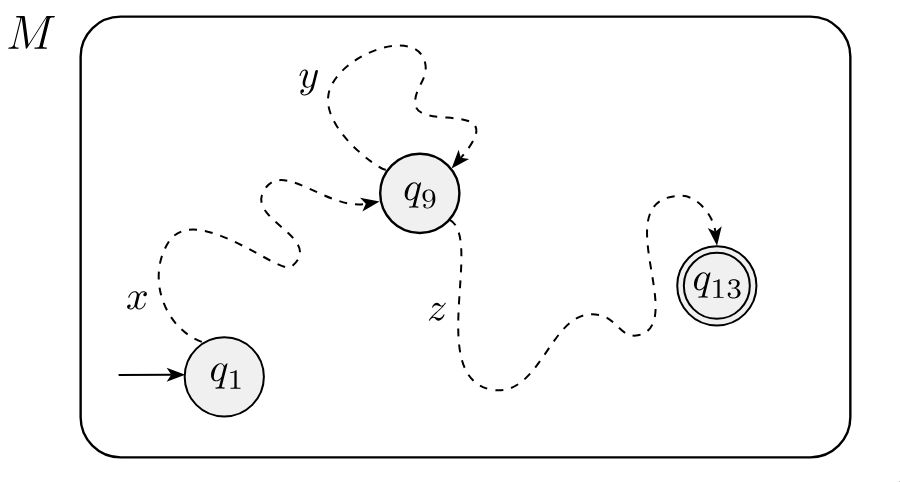
\includegraphics[scale=0.3]{img/2024-12-08-17-37-33.png}
\end{center}

Vediamo perche' questa suddivisione rispetta le tre condizioni. Consideriamo l'input $ xyyz $ passato a $ M $: $ x $ ci porta da $ q_1  $ a $ q_9 $, la prima $ y $ ci porta da $ q_9 $ a $ q_9 $, anche la seconda ci porta da $ q_9 $ a $ q_9 $, infine $ z $ ci porta da $ q_9 $ a $ q_{13} $ (lo stato finale). Quindi $ xyyz $ e' accettato da $ M $, ma anche $ xy^iz $ per lo stesso motivo. Nel caso $ xy^0z $ vediamo che viene riconosciuto anche lui, quidi la prima condizione e' verificata. Dato che $ y $ e' la parte della stringa che ci porta da $ q_9 $ a $ q_9 $, deve essere per forza non nulla perche $ M $ e' deterministico. Infine, la terza condizione e' rispettata dato che, per la \textbf{pigeonhole principle} la prima ripetizione deve avvenire per forza entro i primi $ p+1 $ stati, quindi $ |xy| \leq p $.

\pf{Dimostrazione formale}{
  Sia $ M = (Q, \Sigma, \delta, q_1, F) $ un DFA che riconosce il linguaggio regolare $ A $ e $ p = |Q| $.

  Sia $ s = s_1s_2...s_n $ una stringa in $ A $ tale che $ |s| = n \geq p $ e siano $ r_1, r_2, ..., r_{n+1} $ la sequenza di stati che attraversa $ M $ quando viene dato $ s $ come input, quindi $ r_{i+1} = \delta(r_i, s_i) $. Dato che $ n+1 \geq p+1 $, per il pigeonhole principle fra i primi $ p+1 $ stati ce ne deve essere uno che si ripete. Chimiamo $ r_j $ il primo e $ r_l $ la ripetizione, quindi abbiamo che $ l \leq p+1 $. 

  Ora siano $ x = s_1 ... s_{j-1} $, $ y = s_j ... s_{l-1} $ e $ z = s_l ... s_{n} $. Dato che $ x $ porta $ M $ da $ r_1 $ a $ r_j $, $ y $ porta da $ r_j $ a $ r_l $ e $ z $ porta da $ r_l $ a $ r_{n+1} $ e siccome $ r_j $ e $ r_l $ sono lo stesso stato, $ M $ deve accettare $ xy^iz $ $ \forall i \geq 0 $. Siccome $ j \neq l $, $ |y| > 0 $; e $ l \leq p+1 $, quindi $ |xy| \leq p $. Abbiamo quindi soddisfatto tutte le condizioni del pumping lemma.
}

\subsubsection{Utilizzo ed esempi}
Per dimostrare che $ B $ non e' un linguaggio regolare, prima assumiamo che $ B $ sia regolare e poi dimostriamo che non vale la proprieta' $ P $ del pumping lemma:
\[
\lnot P \implies B \text{ non e' regolare}
\]
Dato che porprio per il lemma, $ B $ e' regolare $ \implies P $. Quindi, bisogna assumere che $ p $ sia la lunghezza garantita dal pumping lemma e prendere una stringa $ s \in B. |s| \geq p $ tale che noi sappiamo che $ z $ non puo' essere pompata. Dimostriamo questo mostrando che per qualunque suddivisione $ xyz $ che rispetti le ultime due condizioni, la prima condizione non vale mai. Solitamente possiamo raggruppare i tipi di suddivisione in diverse categorie che possono essere analizzate individualmente, in modo da non dover controllare davvero ogni suddivisione. Trovando $ s $, abbiamo dimostrato $ \lnot P $ e quindi che $ B $ non e' regolare. 

Per trovare $ s $, solitamente ci vuole un po' di creativita. Bisogna provare a trovare una stringa che raccolga l'"essenza" dell'irregolarita' del linguaggio, vediamo un paio di esempi per chiarire:
\ex{}{
  $ B = \{0^n 1^n \mid n \geq 0\} $
}
\ex{}{
  $ C = \{w \mid w \text{ ha lo stesso numero di 0 e 1}\} $
}
\ex{}{
  $ F = \{ww \mid w \in \{0, 1\}^*\} $
}
TODO: fai esercizi (che sono risolti sul libro)
